\documentclass[11pt, a4paper]{article} %or article has only section and below, book and report also have chapter: http://texblog.org/2007/07/09/documentclassbook-report-article-or-letter/
\usepackage{float}
\usepackage[utf8]{inputenc} % use utf8 encoding of symbols such as umlaute for maximal compatibility across platforms
\usepackage{caption} % provides commands for handling caption sizes etc.
%\usepackage[a4paper, left=25mm, right=20mm, top=25mm, bottom=20mm]{geometry} % to easily change margin widths: https://www.sharelatex.com/learn/Page_size_and_margins
\usepackage[bottom]{footmisc} % I love footnotes! And they should be down at the bottom of the page!
\usepackage{graphicx} % when using figures and alike
\usepackage[hidelinks]{hyperref} % for hyperreferences (links within the document: references, figures, tables, citations)
\usepackage{euler} % a math font, only for equations and alike; call BEFORE changing the main font; alternatives: mathptmx, fourier,
%\usepackage{gentium} % for a different font; you can also try: cantarell, charter, libertine, gentium, bera, ... http://tex.stackexchange.com/questions/59403/what-font-packages-are-installed-in-tex-live
%------------------------------------------------------------------------------------------------------
%------- text size settings --------------
\setlength{\textwidth}{16cm}%
\setlength{\textheight}{25cm} %23
%(these values were used to fill the page more fully and thus reduce the number of pages!)
\setlength{\topmargin}{-1.5cm} %0
\setlength{\footskip}{1cm} %
%\setlength{\hoffset}{0cm} %
\setlength{\oddsidemargin}{1cm}%
\setlength{\evensidemargin}{-.5cm}%
\setlength{\parskip}{0cm} % Abstand zwischen Absätzen
% ----------------------------------------------------------------
\renewcommand{\textfraction}{0.1} % allows more space to graphics in float
\renewcommand{\topfraction}{0.85}
%\renewcommand{\bottomfraction}{0.65}
\renewcommand{\floatpagefraction}{0.70}
\frenchspacing %http://texwelt.de/wissen/fragen/1154/was-ist-french-spacing-was-macht-frenchspacing
%------------------------------------------------------------------------------------------------------
%------------------------------------------------------------------------------------------------------
\usepackage{Sweave}
\begin{document}
\Sconcordance{concordance:alles.tex:alles.Rnw:%
1 28 1 1 3 3 1 1 0 10 1 1 6 16 1 1 2 1 0 10 1 3 0 1 2 %
5 1 1 6 1 18 20 0 1 2 1 1 1 5 1 23 25 0 1 2 2 1 1 2 1 %
0 4 1 3 0 1 2 3 1 1 5 1 2 1 0 3 1 1 3 2 0 4 1 4 0 1 2 %
2 1 1 3 2 0 1 2 1 0 1 1 1 2 1 0 2 1 1 2 1 0 5 1 1 2 5 %
0 1 2 1 1 1 2 16 0 1 2 5 1 1 2 21 0 2 2 1 0 1 1 3 0 1 %
2 8 1 1 2 1 0 5 1 1 2 5 0 1 2 10 1 1 4 3 0 4 1 1 4 3 %
0 1 3 2 0 4 1 1 4 7 0 1 2 16 1 1 2 5 0 1 2 2 1 1 2 4 %
0 1 3 4 0 1 2 1 1 1 3 2 0 2 1 4 0 1 2 5 1 1 2 1 0 3 1 %
4 0 1 2 11 1 1 2 9 0 1 2 4 1 1 5 1 2 4 0 1 2 9 1 1 2 %
1 0 1 1 3 0 1 2 2 1 1 2 1 0 4 1 3 0 2 2 1 0 1 1 3 0 1 %
2 1 1 1 3 35 0 2 2 1 0 2 1 5 0 1 3 6 1 1 2 1 0 1 2 1 %
0 1 1 3 0 2 2 4 0 1 2 138 1 1 2 1 0 1 1 12 0 1 2 14 1 %
1 2 10 1 1 2 6 0 1 1 4 0 1 2 8 1 1 2 1 0 1 1 5 0 1 3 %
8 1 1 2 1 0 3 1 4 0 1 2 8 1 1 2 13 0 2 1 19 0 1 3 8 1 %
1 2 1 0 2 1 5 0 1 3 4 1 1 2 1 0 1 1 5 0 1 3 5 1 1 2 1 %
0 1 1 12 0 1 3 3 1 1 25 3 1 1 2 1 0 2 1 4 0 1 2 9 1 1 %
2 1 0 2 1 5 0 1 3 5 1 1 2 1 0 1 1 10 0 1 2 4 1 1 2 1 %
0 2 1 4 0 1 2 2 1 1 2 1 0 1 1 22 0 2 1 3 0 1 2 1 1 1 %
2 1 0 2 1 5 0 1 4 1 1 1 2 4 0 1 2 1 1 1 2 1 0 1 1 31 %
0 1 1 7 0 2 1 3 0 1 2 2 1 1 2 10 0 1 2 2 1 1 2 6 0 1 %
1 6 0 1 2 2 1 1 2 1 0 1 1 6 0 1 2 5 1 1 2 1 0 1 1 11 %
0 1 2 3 1 1 2 1 0 1 1 1 2 1 0 3 1 1 2 11 0 1 1 1 3 2 %
0 1 1 5 0 1 3 5 1 1 2 1 0 1 1 5 0 1 3 6 1 1 2 1 0 1 1 %
4 0 1 2 7 1 1 2 1 0 1 2 2 1 1 3 2 0 1 2 5 0 1 2 30 1}

\title{Time Series Analysis - A Tutorial}
\author{Rosskopf,E.; Cordes, M.; Lumiko, J.}
% for more control, multiple affiliations, line breaks and alike, use the authblk package!!
\date{\today} % !!use package isodate for more control of date formatting!!
\maketitle
\abstract{Tutorial for time series analysis in R... }
\tableofcontents
\pagebreak
\section{Introduction}%------------------------------------------------------------------------------------
This tutorial assumes that the reader has some basic knowledge of time series analysis, and the principal focus of the tutorial is not to explain time series analysis, but rather to explain how to carry out these analyses using R.
\noindent
If you are new to time series analysis, and want to learn more about any of the concepts presented here, We would highly recommend the Open University book “Time series” (product code M249/02), available from from the Open University Shop.
%\begin{itemize}
%\item Definition time series\\
%\item examples in economy, nature, humans,.... \\
%\item stochastic/deterministic with dormann revision\\
%\item stationary / non stationary \\
%\item regression: why time series regression instead of linear standrard regression\\
%\item where you need to use time series regression.\\
%\end{itemize}
\section{Getting started}%------------------------------------------------------------------------------------
\subsection{Packages}
Before we get started, please make sure to set a working directory and download the necessary packages listed below.\\
\noindent Useful packages for time series analysis:
\begin{Schunk}
\begin{Sinput}
> library(tseries)
> library(nlme)
> library(car)
> library(knitr)
> library(xtable)
> library(SweaveListingUtils)
> library(stats)
> library(forecast)
> library(AICcmodavg)
> library(TTR)
> library(mgcv)
\end{Sinput}
\end{Schunk}
\subsection{Functions needed lateron}
function writing to organize our script:\\
\noindent first we can write a diagnostics function with all the tests we need to perform to check if our model is adequate enough to stop the model adaptation.\\
we need to be careful if we want to check for residuals or the whole model.
so x will be the model and x$residuals and x$fitted are the other options we need.\\
\begin{Schunk}
\begin{Sinput}
> diagnostics <- function (x)
+ {
+ normality = shapiro.test(x$residuals); #check for normal distributed values #
+ stat.res = adf.test(x$residuals); #check both residuals and fitted of the model for stationarity
+ stat.fit = adf.test(x$fitted);
+ x$residualsvector = as.vector(x$residuals);
+ autocorr= dwt(x$residualsvector) ; #check for autocorrelation
+ indep= Box.test(x$residuals, type="Ljung-Box") #check for independence
+ #lag for season is df: m-1 ( 12-1)
+ #write if seasonal = TRUE lag=12-1, else write nothing
+ #there is high evidence that there are non-zero autocorr.
+ output = list(normality, stat.res, stat.fit, autocorr, indep)
+ names (output) = c("norm. distrb. of residuals", "stationarity of residuals", "stationarity of fitted values", "autocorrelation of residuals", "independence of residuals")
+ return ( output )
+ }
\end{Sinput}
\end{Schunk}
\noindent Lateron for the forecast plotting, we need the histogram with the normal distribution to see wether the errors of the forecast model are well distributed:
\begin{Schunk}
\begin{Sinput}
> plotForecastErrors <- function(forecasterrors)
+ {
+ # make a histogram of the forecast errors:
+ mybinsize <- IQR(forecasterrors)/4
+ mysd <- sd(forecasterrors)
+ mymin <- min(forecasterrors) - mysd*5
+ mymax <- max(forecasterrors) + mysd*3
+ # generate normally distributed data with mean 0 and standard deviation mysd
+ mynorm <- rnorm(10000, mean=0, sd=mysd)
+ mymin2 <- min(mynorm)
+ mymax2 <- max(mynorm)
+ if (mymin2 < mymin) { mymin <- mymin2 }
+ if (mymax2 > mymax) { mymax <- mymax2 }
+ # make a red histogram of the forecast errors, with the normally distributed data overlaid:
+ mybins <- seq(mymin, mymax, mybinsize)
+ hist(forecasterrors, col="red", freq=FALSE, breaks=mybins)
+ # freq=FALSE ensures density
+ # generate normally distributed data with mean 0 and standard deviation mysd
+ myhist <- hist(mynorm, plot=FALSE, breaks=mybins)
+ # plot the normal curve as a blue line on top of the histogram of forecast errors:
+ points(myhist$mids, myhist$density, type="l", col="blue", lwd=2)
+ }
\end{Sinput}
\end{Schunk}
\subsection{Dataset (CO2-Concentrations)}%------------------------------------------------------------------------------------
The first dataset we will work with consists of monthly CO2-concentrations [ppm] in the atmosphere, measured over time at the famous Mauna Loa Station on Hawaii.\\
To download this dataset, just use the code provided below.
\begin{Schunk}
\begin{Sinput}
> url<-"ftp://aftp.cmdl.noaa.gov/products/trends/co2/co2_mm_mlo.txt"
> dest<-"C:/Users/Mallypop/Desktop/AllInclusive/co2_mm_mlo.txt"
> download.file(url, dest )
> co2month=read.table(dest, skip=72)
> co2month
\end{Sinput}
\end{Schunk}
\noindent Note:"dest'' represents a randomly chosen name for a text file in which the CO2-dataset will be saved. Feel free to adjust the name and directory.
\subsection{Dataset Visualization}%-----------------------------------------------------------------------------------
It can be really useful to visualize your dataset before you transform it into a timeseries (ts) in order to detect potential errors.
\subsubsection{Histogram \& QQ-Plot}
\begin{Schunk}
\begin{Sinput}
> data = co2month[,c(3,5)]
> colnames(data)= c("year", "co2")
> attach(data)
> x = co2
> op = par(mfrow = c(1,2),
+ mar = c(5,4,1,2)+.1,
+ oma = c(0,0,2,0))
> hist(co2, freq=F, col = "cornsilk",xlab = "", main = "")
> qqnorm(x, main = ""); qqline(x,col = 'red')
> par(op)
> mtext("CO2 Concentration (ppm) Histogram and QQ Plot", line = 2.5,font = 2,cex = 1.0)
\end{Sinput}
\end{Schunk}
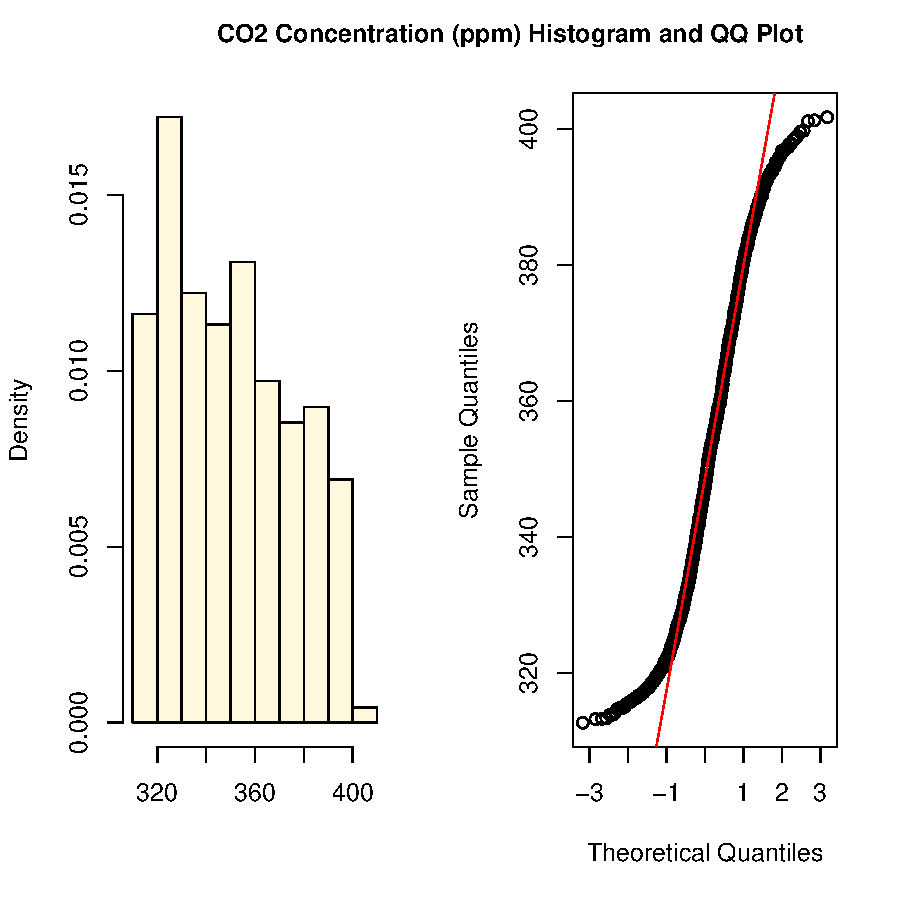
\includegraphics{alles-fig1check}
\subsubsection{Plotting the fitted values}
\begin{figure}[H]
\centering
\begin{Schunk}
\begin{Sinput}
> # Run a linear model
> datalm = lm( co2 ~ year)
> # Fit predict values
> MyData=data.frame(year=seq(from=(1958),to=2014, by=0.1))
> pred=predict(datalm, newdata=MyData, type="response", se=T)
> # Plot the fitted values
> plot(year, co2, type="n",las=1, xlab="Year", ylab="CO2 conc. (ppm)", main="CO2 concentration in the atmosphere")
> grid (NULL,NULL, lty = 6, col = "cornsilk2")
> points(year, co2, col="cornflowerblue" )
> # Write confidence interval
> F=(pred$fit)
> FSUP=(pred$fit+1.96*pred$se.fit) # make upper conf. int.
> FSLOW=(pred$fit-1.96*pred$se.fit) # make lower conf. int.
> lines(MyData$year, F, lty=1, col="red", lwd=3)
> lines(MyData$year, FSUP,lty=1, col="red", lwd=3)
> lines(MyData$year, FSLOW,lty=1, col="red", lwd=3)
> legend("topleft",c("simple linear regression y~x", "monthly mean data"),
+ pch=c(20,20), col=c("red", "cornflowerblue"))
\end{Sinput}
\end{Schunk}
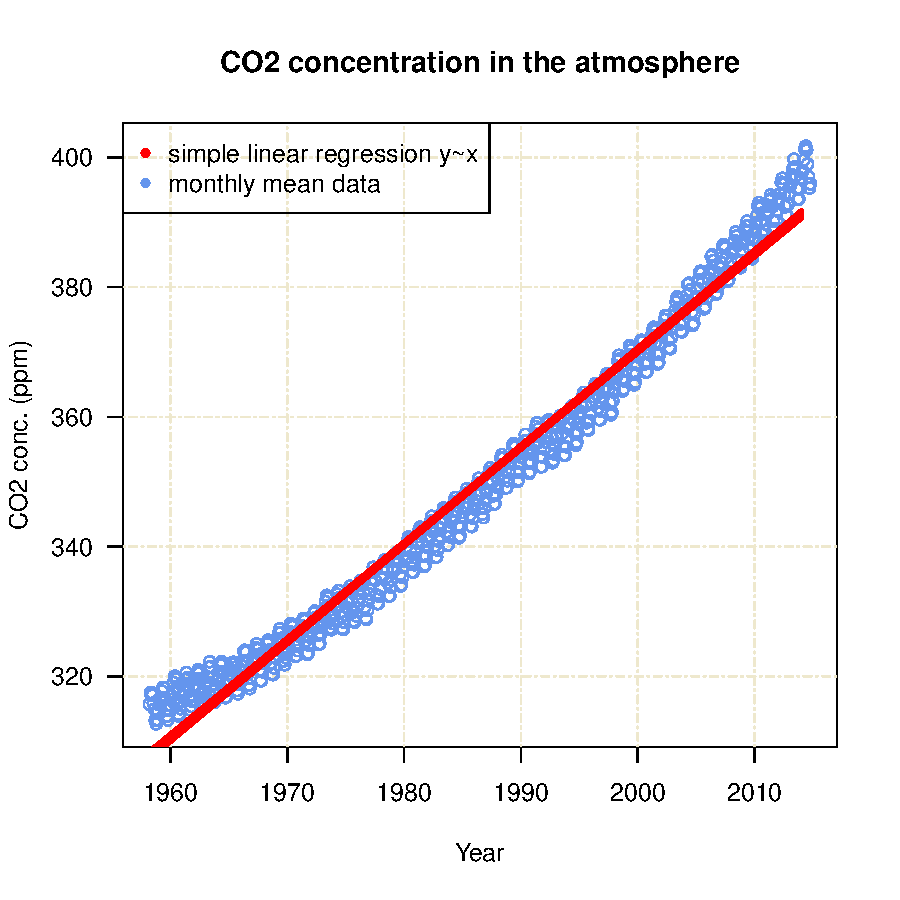
\includegraphics{alles-fig1datalm}
\end{figure}
Look at standard errors, highly underestimated, standard errors are higher in true ! p value is not right evidence , misleading :
\begin{Schunk}
\begin{Sinput}
> xtable(summary(datalm))
\end{Sinput}
% latex table generated in R 3.1.2 by xtable 1.7-4 package
% Wed Nov 26 11:00:02 2014
\begin{table}[ht]
\centering
\begin{tabular}{rrrrr}
  \hline
 & Estimate & Std. Error & t value & Pr($>$$|$t$|$) \\ 
  \hline
(Intercept) & -2618.5566 & 16.9782 & -154.23 & 0.0000 \\ 
  year & 1.4944 & 0.0085 & 174.86 & 0.0000 \\ 
   \hline
\end{tabular}
\end{table}\end{Schunk}
\noindent This plot (~\ref{fig1datalm} can be used to observe if there are outliers which could possibly bias the model. \\
However the poly-1 linear regression is not accurate in fitting the CO2-dataset. This is due to the present autocorrelation that not yet has been taken into account. Neglecting this factor will always effect the accuracy of the model results. The standard errors are lower than their true values thus giving high statistical significance with a p-value lower than it should be. The clue in statistical modelling is to present the correct statistical evidence, which would be highly biased with a linear model.\\
\subsection{Dataset Transformation}
It is essential to transform your dataset into a timeseries (ts) if you seek for an accurate and extensive analysis of the data.
\noindent The data stored as a dataframe needs to be transformed with the important columns into the class of a time series to continue working on it properly. If you have monthly data you have to set the deltat of the function ts() to deltat=1/12 describing the sampling period parts between successive values xt and xt+1. Your time series should somehow look like table 1.\\
\noindent \textbf{Original Data}\\
\begin{Schunk}
\begin{Sinput}
> xtable(head(data), caption="Original CO2-Data")
\end{Sinput}
% latex table generated in R 3.1.2 by xtable 1.7-4 package
% Wed Nov 26 11:00:02 2014
\begin{table}[ht]
\centering
\begin{tabular}{rrr}
  \hline
 & year & co2 \\ 
  \hline
1 & 1958.21 & 315.71 \\ 
  2 & 1958.29 & 317.45 \\ 
  3 & 1958.38 & 317.50 \\ 
  4 & 1958.46 & 317.10 \\ 
  5 & 1958.54 & 315.86 \\ 
  6 & 1958.62 & 314.93 \\ 
   \hline
\end{tabular}
\caption{Original CO2-Data} 
\end{table}\end{Schunk}
\noindent \textbf{Transformation}\\
\begin{Schunk}
\begin{Sinput}
> yourts=ts(co2, c(1958,3),c(2014,10), deltat=1/12)
> class(yourts)
\end{Sinput}
[1] "ts"\end{Schunk}
%<<results=tex, echo=FALSE, print=TRUE >>=
%print(xtable(yourts, digits=2, label="yourts",caption="Your time series for monthly mean data"), size="\\tiny")
%@
%\pagebreak
\subsection{Time-Series Visualization}%------------------------------------------------------------------------------------
It is important to get a quick overview of your data. Some simple plots for visualization are quite helpful.
\subsubsection{Time-Series Plot}
\begin{figure}[H]
\centering
\begin{Schunk}
\begin{Sinput}
> par(mfrow=c(1,1))
> plot.ts(yourts,las=1, xlab="Year", ylab="CO2 conc. (ppm)", main="CO2 concentration in the atmosphere")
> grid (NULL,NULL, lty = 6, col = "cornsilk2")
> points(yourts, col="cornflowerblue" )
> k <- 5
> lines(year,filter(co2, rep(1/k,k) ),col = 'red', type="l", lwd = 3)
> legend("topleft",c("simple moving average", "monthly mean data"),
+ pch=c(20,20), col=c("red", "cornflowerblue"))
\end{Sinput}
\end{Schunk}
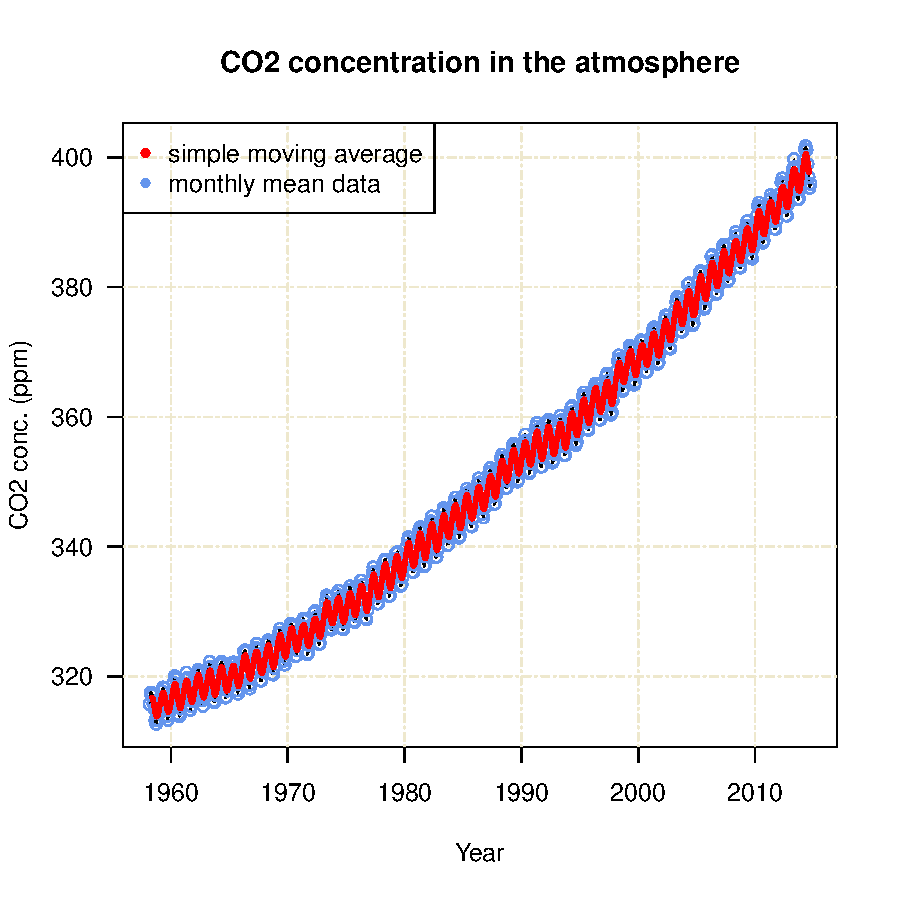
\includegraphics{alles-fig1visualize}
\caption{Visualization of the CO2 Concentrations}
\label{fig1visualize}
\end{figure}
\noindent \textbf{Note: The red line in plot \ref{fig1visualize} was computed with a simple moving average. It is not enough to just run a MA.}\\
%\pagebreak
\subsubsection{ACF, PACF, SPECTRUM}
\noindent Since time-series data usually violates the independence assumption of the model, the standard error is potentially too small. As the data are regularly spaced in time, we can easily employ the autocorrelation function to investigate residuals correlations in the model errors.\\
\textbf{The acf() function} can be used for that, which produces a plot of the correlogram.\\
Another nice procedure is to run the \textbf{autocorrelation function} with its complementary \textbf{partial acf} and the \textbf{spectrum} showing the spectral density of your time series at frequencies corresponding to the possibly approx. Fourier frequencies. \\
\begin{figure}[H]
\centering
\begin{Schunk}
\begin{Sinput}
> op <- par(mfrow = c(3,1),
+ mar = c(2,4,1,2)+.1,
+ oma = c(0,0,2,0))
> acf(x, xlab = "")
> pacf(x, xlab = "")
> spectrum(x, xlab = "", main = "")
> par(op)
> mtext("CO2 Concentration (ppm) correlogram",
+ line = 2.5,
+ font = 2,
+ cex = 0.8)
> op <- par(mfrow = c(3,1),
+ mar = c(2,4,1,2)+.1,
+ oma = c(0,0,2,0))
> acf(resid(datalm), xlab = "")
> pacf(resid(datalm),xlab = "")
> spectrum(resid(datalm), xlab = "", main = "")
> par(op)
> mtext("Model residual correlogram",
+ line = 2.5,
+ font = 2,
+ cex = 1.2)
\end{Sinput}
\end{Schunk}
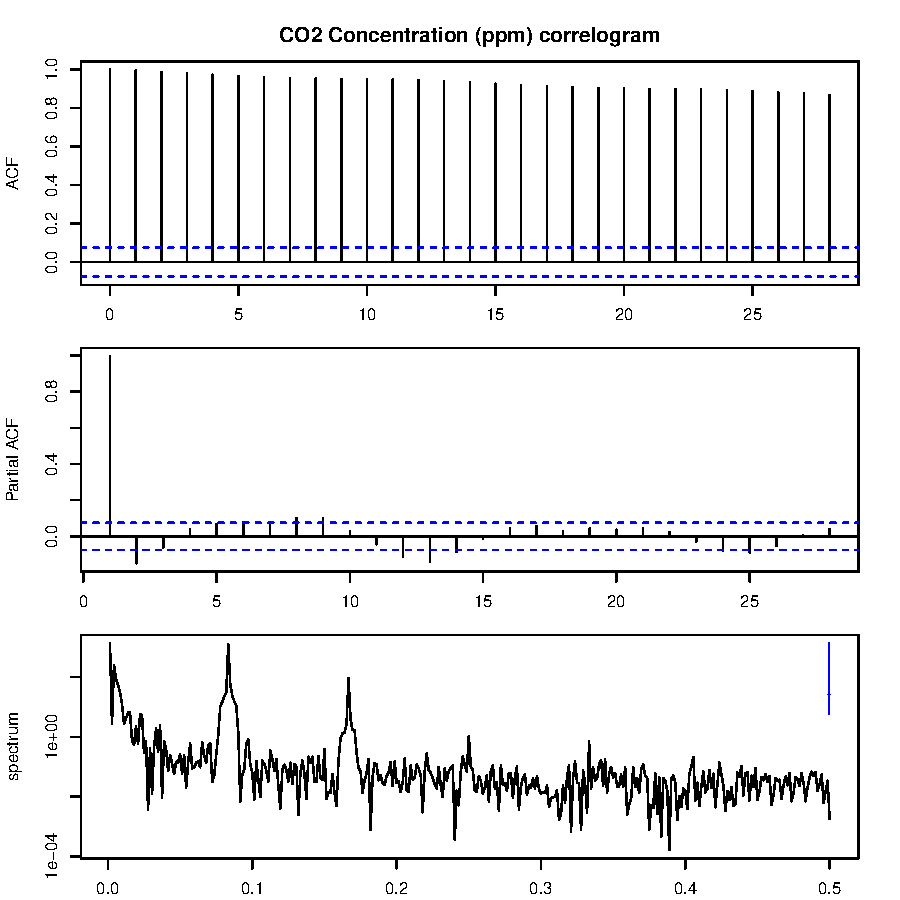
\includegraphics{alles-correlogram}
\caption{Correlogram of time series and residuals of lm}
\label{correlogram}
\end{figure}
Explain the acf , pacf, spectrum here. \\
\textbf{ACF \& PACF:}\\
\noindent The generated correlogram reveals that there are major autocorrelations. \\
There is a strong correlation at lag 1,a weaker correlation at lag 2, and a noticeable correlation at lag 3. Such a correlation pattern is typical for an autoregressive process where most of the sequential dependence can be explained as a flow-on effect from a dependence at lag 1.\\
\noindent In an autoregressive time series, an independent error component, or ''innovation" is associated with each time point. For an order p autoregressive time series, the error for any time point is obtained by taking the innovation for that time point, and adding a linear combination of the innovations at the p previous time points. (For the present time series, initial indications are that p = 1 might capture most of the correlation structure.)"\\ (autosmooth.pdf)\\
\noindent \textbf{Spectrum:} easier to interpret the acf / log scaled / strong cycles where spectrum max. occurs
Here the highest maximum is at about 0.75. 1/0.75 = 12 meaning a 12 month cycle is occuring here .\\
\noindent The residuals in a time series are serially correlated. The ACF is waving and decreases only slowly, which could be an identification of non-stationarity ( If the ACF would drop to zero quickly, the time series would be stationary). We stop all diagnostics here for our clearly wrong model and go on to investigate the different components of our time series.\\
\section{Decomposition of Time Series}%-----------------------------------------------------------------------------------------------------
A time serie consists of 3 components; a trend component, an irregular (random) component and (if it is a seosonal time series) seasonal component.
\subsection{Decomposing Seasonal Data}%----------------------------------------------------------------------------------------------------
\noindent We can decompose the ts and plot these components:
\begin{figure}[H]
\centering
\begin{Schunk}
\begin{Sinput}
> plot(decompose(yourts))
\end{Sinput}
\end{Schunk}
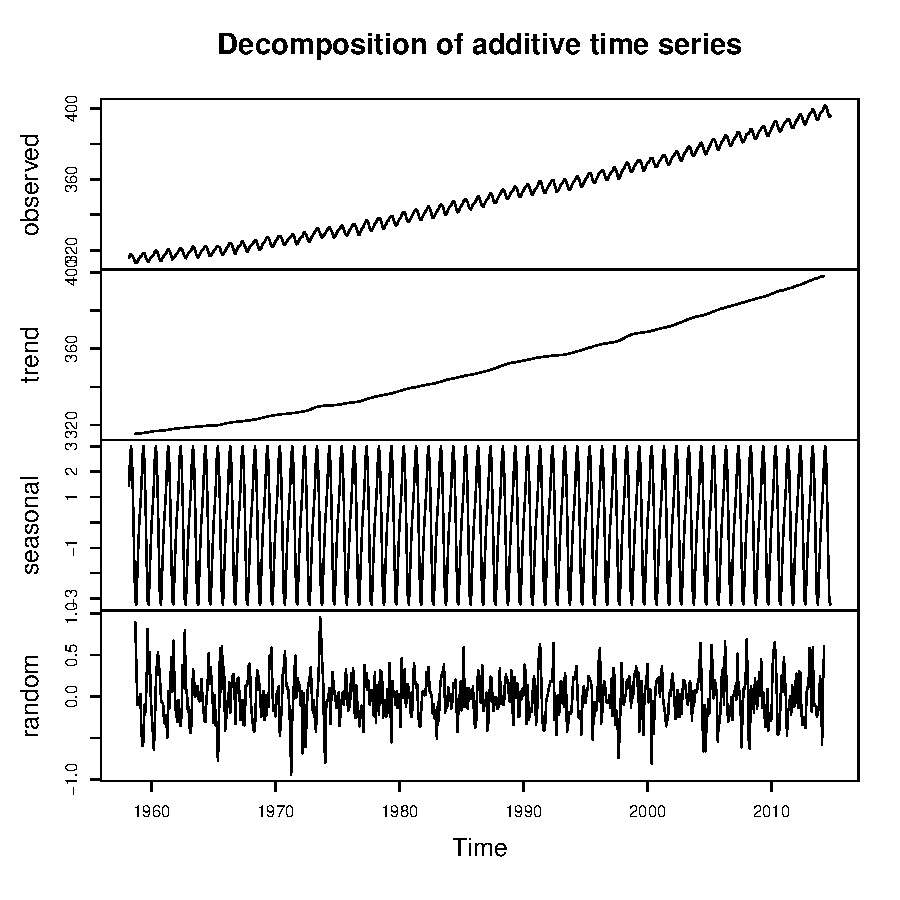
\includegraphics{alles-decompose}
\caption{Decomposition of the CO2 Time Series}
\end{figure}
\noindent We can see each component with:
\begin{Schunk}
\begin{Sinput}
> yourts_components<- decompose(yourts)
\end{Sinput}
\end{Schunk}
\begin{Schunk}
\begin{Sinput}
> yourts_components$seasonal
\end{Sinput}
\end{Schunk}
\begin{figure}[H]
\centering
\begin{Schunk}
\begin{Sinput}
> #we can see the trend for the first year:
> par(mfrow=c(1,2))
> ts.plot(yourts_components$seasonal[1:12])
> ts.plot(aggregate(yourts_components$seasonal))
\end{Sinput}
\end{Schunk}
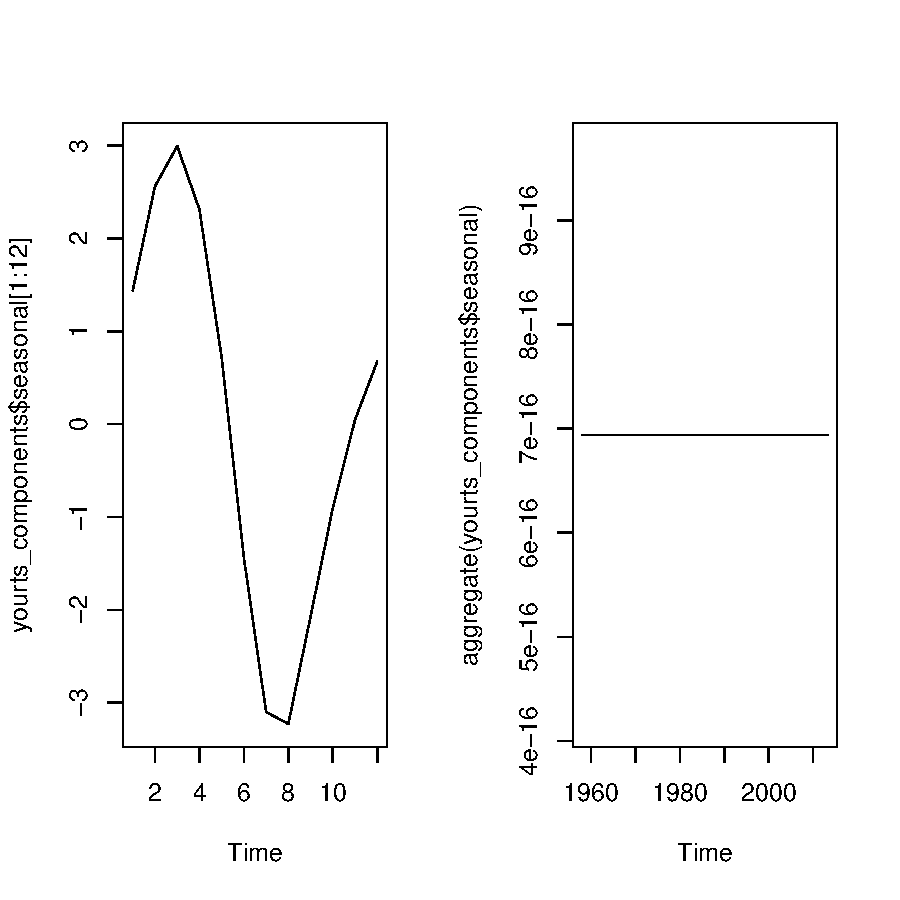
\includegraphics{alles-decomposition}
\caption{The seasonal component across the time}
\label{decomposition}
\end{figure}
It seems that our seasonal component is positive until the summer months, were it turns to be negative and turning to be positiv again in winter (see fig. ~\ref{decomposition}). And we can see in the right plot that this seasonal component is constant over all the years (see fig. ~\ref{decomposition}).
\begin{figure}[H]
\centering
\begin{Schunk}
\begin{Sinput}
> yourts_seasonallyadjusted <- yourts - yourts_components$seasonal
> par(mfrow=c(1,2))
> plot(yourts, main="TS with seasonal fl.", las=1)
> plot(yourts_seasonallyadjusted, las=1, main="removed seasonal fluctuation")
\end{Sinput}
\end{Schunk}
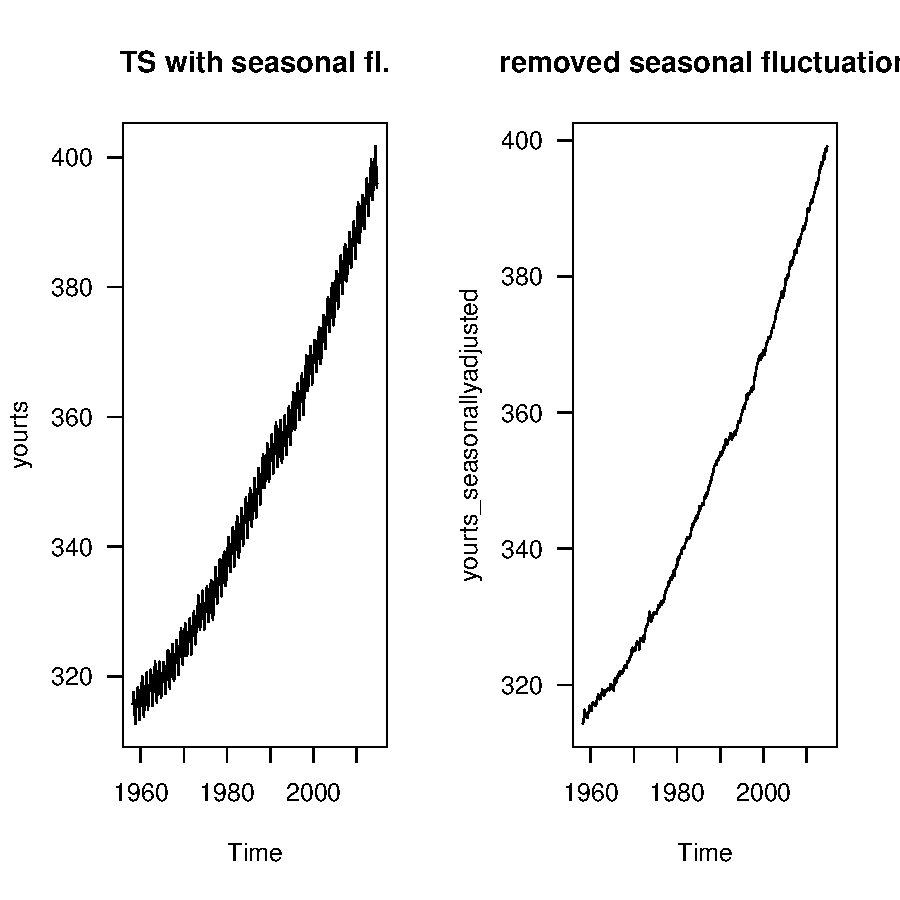
\includegraphics{alles-seasonallyadjusted}
\caption{Comparison of seasonal vs. seasonally adjusted model}
\label{decomposition2}
\end{figure}
\noindent It seems that our data can probably be described using an additive model, since the random fluctuations in the data are roughly constant in size over time (constant seasonal component). In some cases it might be handy to have the model without the seasonal fluctuations to depict change in the trend and local extremes easier (see fig. ~\ref{decomposition2}).
\section{Analysis of Seasonal Data}
After looking at the simple linear regression datalm, we were facing some serious problems with our model.
To be sure about non-stationarity of our time series, wen can run the adf.test, giving us the result that our data is non-stationary and we need to fix it:
\begin{Schunk}
\begin{Soutput}
	Augmented Dickey-Fuller Test

data:  yourts
Dickey-Fuller = -1.0663, Lag order = 8, p-value = 0.928
alternative hypothesis: stationary
\end{Soutput}
\end{Schunk}
Also we need a model which is covering the serial correlation of our residuals. The ACF, PACF, spectrum above gives us certainty an the autocorrelation and the seasonality.
The standard errors are highly underestimated, thus in the summary the p-value is too small and misleading.
A nice model to try is GLS, which will allow for correlation of standard errors and unequel variances.
In the GLS we have different options to choose, though our data is not spatially correlated we are not discussing spatial autocorrelation here ( further reading on:...)
Our first try on gls will be simple:
\begin{Schunk}
\begin{Sinput}
> data.glsAR = gls(co2 ~ year,cor= corAR1(acf(resid(datalm))$acf[2]))
> save(data.glsAR, file="data.glsAR.RData")
\end{Sinput}
\end{Schunk}

\begin{Schunk}
\begin{Sinput}
> load("data.glsAR.RData")
\end{Sinput}
\end{Schunk}

The difference will be made in the correlation structure. There are generally ( for temporal corr. interesting) five options you have:
\begin{enumerate}
\item corAR1: in ACF exponential decreasing values of correlation with time distance\\
\item corARMA: either autoregressive order or moving average order or both\\
\item corCAR1: continuous time ( time index does nto have to be integers)\\
\item corCompSymm: correlation does not decrease with higher distance\\
\item corSymm: general correlation only for few observations only, often overparameterized\\
\end{enumerate}
Our first gls model accounts for the AR1, which is clearly visible in the PACF.
\begin{Schunk}
\begin{Sinput}
> acf(data.glsAR$residuals)
\end{Sinput}
\end{Schunk}
We have still a lot of problems concerning the autocorrelation and the seasonality. One option is to allow the AR to use more parameters and/or to include a moving average or error variance to the model. This can be handled via the corARMA. We tried 2 versions, one with 1 lag and 1 moving average, the other with 2 lags and 2 moving averages.
The 0.2 are starting values for Phi, which are in the modelling process optimized.
The next models are thus:
\begin{Schunk}
\begin{Sinput}
> data.glsARMA1 = gls ( co2 ~ year, cor = corARMA (c(0.2,0.2),p=1, q=1 ))
> data.glsARMA2 = gls (co2 ~year, cor=corARMA(c(0.2,0.2,0.2, 0.2), p=2, q=2))
> xtable(anova(data.glsAR, data.glsARMA1, data.glsARMA2))
> save(data.glsARMA1, file="data.glsARMA1.RData")
> save(data.glsARMA2, file="data.glsARMA2.RData")
\end{Sinput}
\end{Schunk}

\begin{Schunk}
\begin{Sinput}
> load("data.glsARMA1.RData")
> load("data.glsARMA2.RData")
\end{Sinput}
\end{Schunk}

% To compare all the models we use anova and the best model is so far the data.glsARMA2 with the lowest AIC and significantly better than the ARMA1, which is itself significantly better than the data.glsAR.
% <<results=tex, echo=FALSE>>=
% #run diagnostics
print(diagnostics(data.glsARMA2))
\begin{figure}[H]
\begin{Schunk}
\begin{Sinput}
> par(mfrow=c(1,2))
> plot(datalm)
> plot(data.glsARMA2)
> #well spread is already smaller of variances
\end{Sinput}
\end{Schunk}
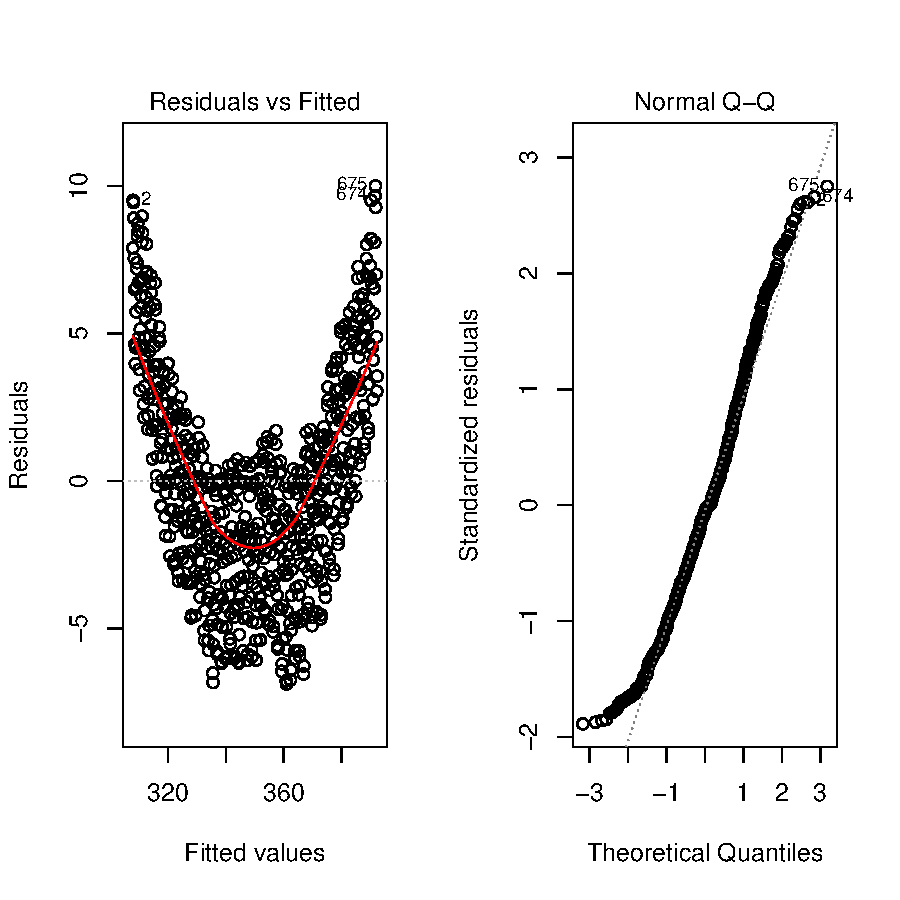
\includegraphics{alles-residual}
\caption{Residuals fitted vs. observed}
\label{residual}
\end{figure}\\

\noindent function writing: if anova$AIC lowest, choose this as bestmodel
But still we have seasonal problems here. We should therefore include a seasonal term.
Try to fit for seasonal component and autocorrelation with best corstruct:
\begin{Schunk}
\begin{Sinput}
> seas = cycle(yourts)
> dataseasongls = gls(co2 ~ year + factor(seas), cor=corARMA( c(0.2,0.2,0.2, 0.2),
+                 p=2, q=2)) #use bestmodel corstruct
> save(dataseasongls, file="dataseasongls.RData")
\end{Sinput}
\end{Schunk}

\begin{Schunk}
\begin{Sinput}
> load("dataseasongls.RData")
\end{Sinput}
\end{Schunk}

\section{Modelling the time series}
The best model for a time series needs to have residuals as white noise terms.
There are different ways to approach this task.
\section{Forecasts}%----------------------------------------------------------------------------------------------------
We have three different options to make ( up to now)
\begin{enumerate}
\item predict
\item Holt Winters
\item Arima forecasts
\end{enumerate}
\subsection{Holt-Winters Exponential Smoothing}%-----------------------------------------------------------------------------------------------
If we have a time series that can be described using an additive model,we can short-time forecast using exponential smoothing.\\
Preconditions:forecast errors are uncorrelated and are normally distributed with mean zero and constant variance.
\begin{Schunk}
\begin{Sinput}
> hw<-HoltWinters(yourts)
> #the alpha value tells us the weight of the previous values for the forecasting
> #values of alpha that are close to 0 mean that little weight is placed on the most recent observations when making forecasts of future values
> #gamma is for the seasonality
> plot(hw)
\end{Sinput}
\end{Schunk}
\noindent Holtwinters just makes forecasts for the time period covered by the original data.If we want to forecast for the future, we need the packeged "forecast".\\
\begin{figure}[H]
\centering
\begin{Schunk}
\begin{Sinput}
> hw1<- forecast.HoltWinters(hw, h=12)
> #for the next year
> plot.forecast(hw1, main="Prediction for the next year",shadecols = "oldstyle")
> #for next 10 years
> hw10<- forecast.HoltWinters(hw, h=120)
> plot.forecast(hw10, main="Prediction for the next 10 years", shadecols = "oldstyle")
\end{Sinput}
\end{Schunk}
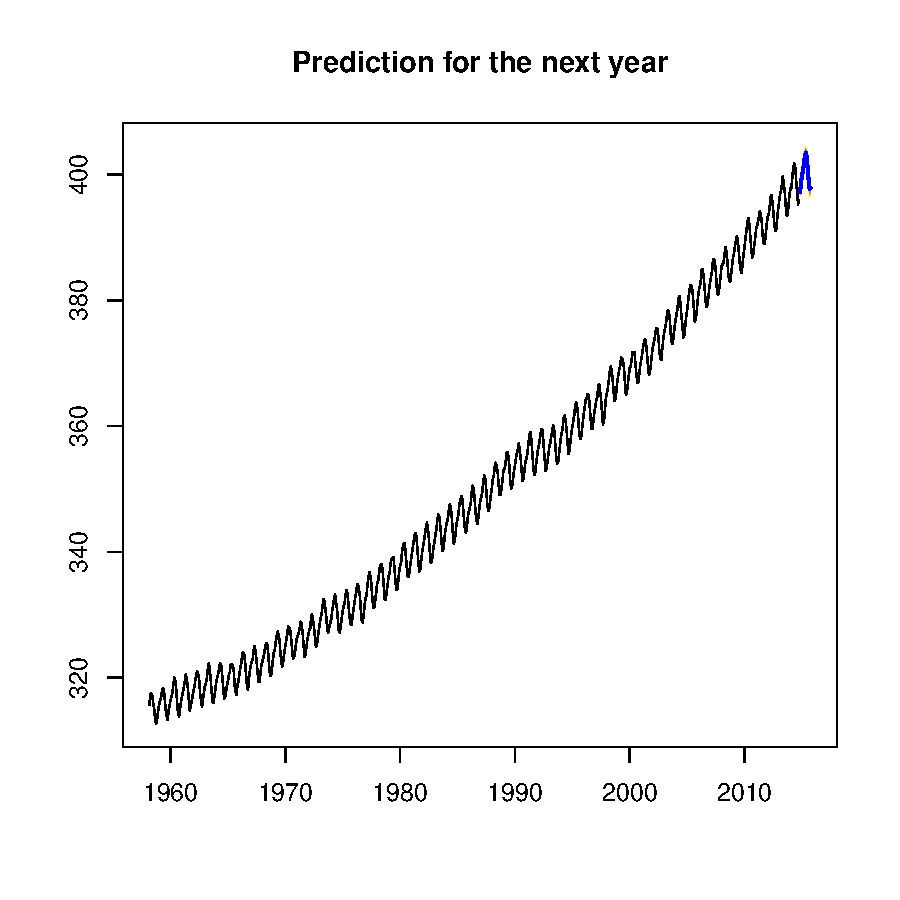
\includegraphics{alles-027}
\caption{Forecasting using Holt Winters exponential smoothing}
\end{figure}
\noindent Here the forecasts for 1913-1920 are plotted as a blue line, the 80% prediction interval as an orange shaded area, and the 95% prediction interval as a yellow shaded area.
\noindent The ‘forecast errors’ are calculated as the observed values minus the predicted values, for each time point. We can only calculate the forecast errors for the time period covered by our original time series. One measure of the accuracy of the predictive model is the sum-of-squared-errors (SSE) for the in-sample forecast errors.
\noindent To calculate a correlogram of the in-sample forecast errors for the CO2 Time series data for lags 1-20, we type:
\begin{figure}[H]
\centering
\begin{Schunk}
\begin{Sinput}
> acf(hw10$residuals, lag.max=20)
\end{Sinput}
\end{Schunk}
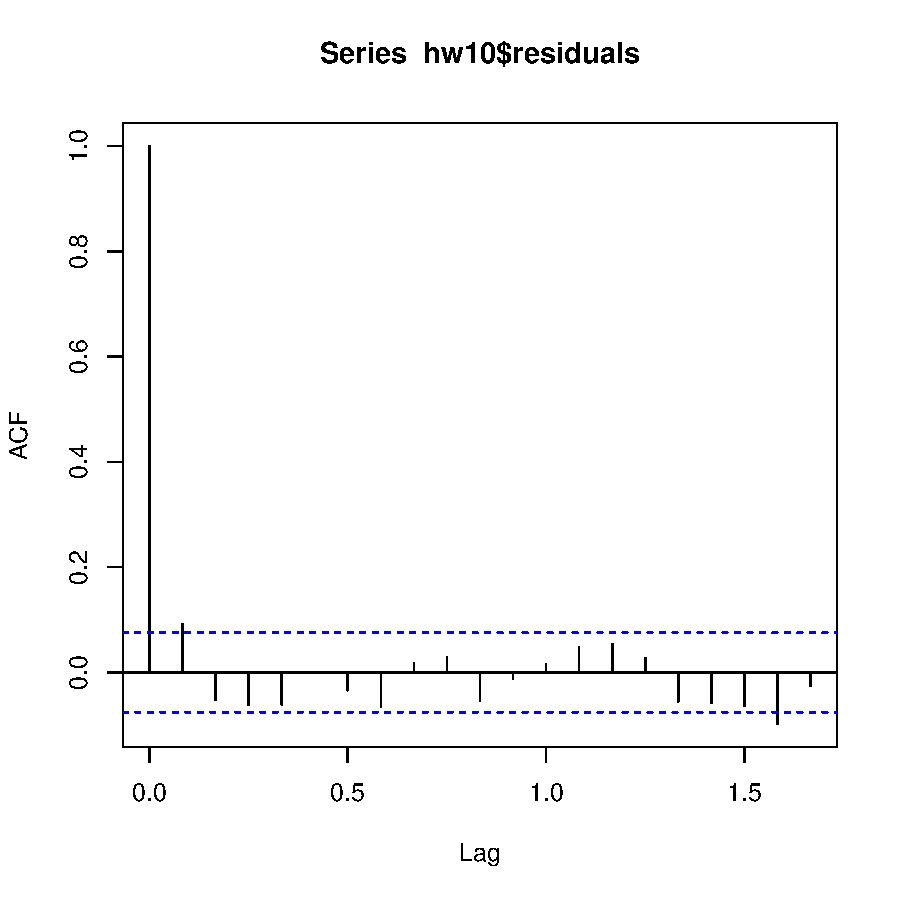
\includegraphics{alles-028}
\caption{Correlogram of the residuals.}
\end{figure}
\begin{Schunk}
\begin{Sinput}
> Box.test(hw10$residuals, lag=20, type="Ljung-Box")
\end{Sinput}
\begin{Soutput}
	Box-Ljung test

data:  hw10$residuals
X-squared = 37.5445, df = 20, p-value = 0.01006
\end{Soutput}
\end{Schunk}
There is little evidence of non-zero autocorrelations at lags 1-20.
\begin{Schunk}
\begin{Sinput}
> plotForecastErrors <- function(forecasterrors)
+ {
+ # make a histogram of the forecast errors:
+ mybinsize <- IQR(forecasterrors)/4
+ mysd <- sd(forecasterrors)
+ mymin <- min(forecasterrors) - mysd*5
+ mymax <- max(forecasterrors) + mysd*3
+ # generate normally distributed data with mean 0 and standard deviation mysd
+ mynorm <- rnorm(10000, mean=0, sd=mysd)
+ mymin2 <- min(mynorm)
+ mymax2 <- max(mynorm)
+ if (mymin2 < mymin) { mymin <- mymin2 }
+ if (mymax2 > mymax) { mymax <- mymax2 }
+ # make a red histogram of the forecast errors, with the normally distributed data overlaid:
+ mybins <- seq(mymin, mymax, mybinsize)
+ hist(forecasterrors, col="red", freq=FALSE, breaks=mybins)
+ # freq=FALSE ensures the area under the histogram = 1
+ # generate normally distributed data with mean 0 and standard deviation mysd
+ myhist <- hist(mynorm, plot=FALSE, breaks=mybins)
+ # plot the normal curve as a blue line on top of the histogram of forecast errors:
+ points(myhist$mids, myhist$density, type="l", col="blue", lwd=2)
+ }
\end{Sinput}
\end{Schunk}
\begin{figure}[H]
\centering
\begin{Schunk}
\begin{Sinput}
> plotForecastErrors(hw10$residuals)
\end{Sinput}
\end{Schunk}
\caption{Histogram of the errors}
\end{figure}
\noindent The histogram of the time series shows that the forecast errors are roughly normally distributed and the mean seems to be close to zero.

\subsection{Seasonal Decomposition of Time Series by Loess}
Forecasting using stl objects:
\begin{figure}[H]
\centering
\begin{Schunk}
\begin{Sinput}
> plot(stlf(yourts, lambda=0, h =120))
> (tslm(yourts~time(yourts)))
\end{Sinput}
\begin{Soutput}
Call:
lm(formula = formula, data = "yourts", na.action = na.exclude)

Coefficients:
 (Intercept)  time(yourts)  
   -2618.494         1.494  
\end{Soutput}
\end{Schunk}
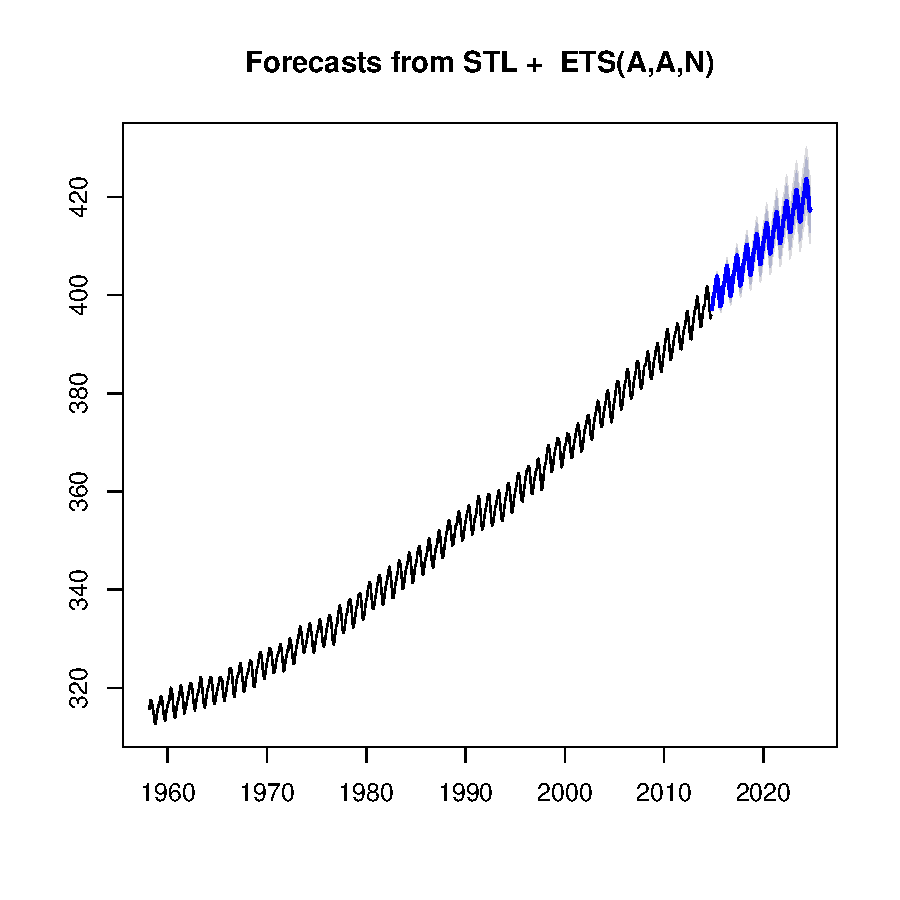
\includegraphics{alles-032}
\caption{Forecasting using Loess}
\end{figure}
\subsection{ARIMA Models}%-----------------------------------------------------------------------------------------------
For the CO2 time series:
\begin{Schunk}
\begin{Sinput}
> au=auto.arima(yourts, ic = "bic")
> arima1=arima(yourts, order = c(au$arma[1],au$arma[6],au$arma[2]))
> fore1=forecast.Arima(arima1,h=10)
> plot.forecast(fore1)
\end{Sinput}
\end{Schunk}
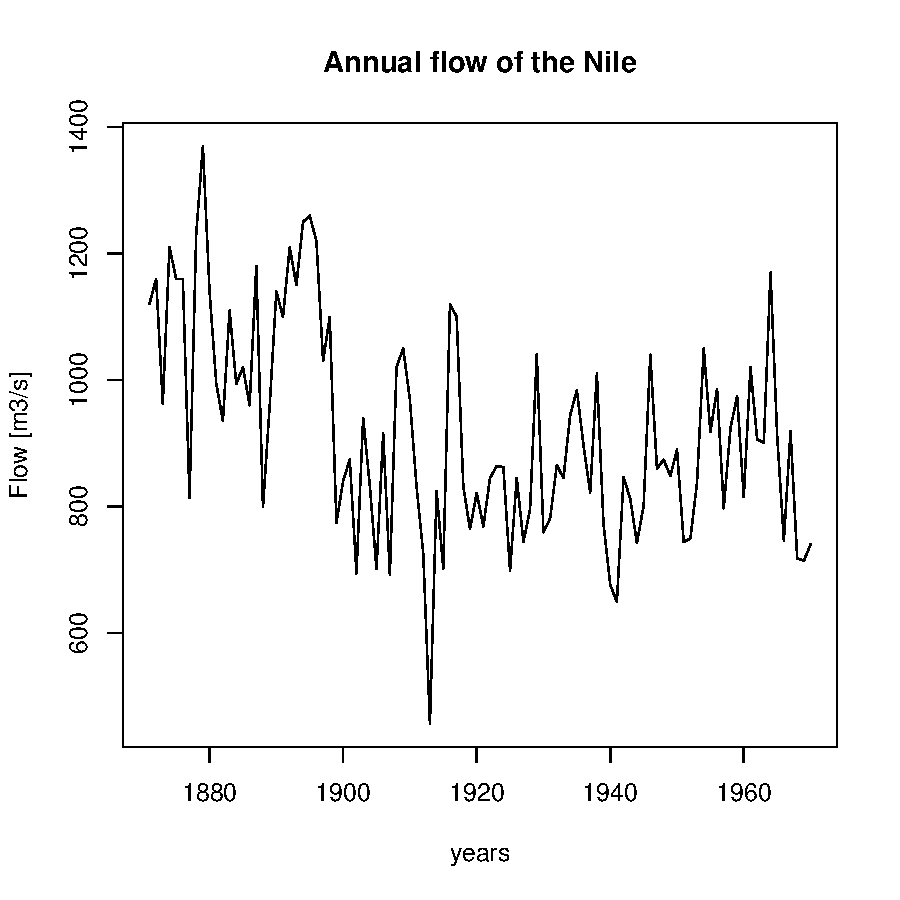
\includegraphics{alles-033}

\subsection{Selecting a Candidate ARIMA Model}%-----------------------------------------------------------------------------------------------
TEXT
\subsection{Forecasting Using an ARIMA Model}%-----------------------------------------------------------------------------------------------
compare both functions of forecasting:
\begin{figure}[H]
\centering
\begin{Schunk}
\begin{Sinput}
> par(mfrow=c(1,2))
> plot(forecast.arima, xlim=c(2010,2025), ylim=c(385,430))
> plot.forecast(forecasts2 ,xlim=c(2010,2025), ylim=c(385,430))
\end{Sinput}
\end{Schunk}
\caption{Model Comparisons}
\end{figure}

\section{Nile}
\subsection{the Nile River Time Series}%------------------------------------------------------------------------------------------------------

\noindent Our example 2 contains the Measurements of the annual flow of the river Nile [m3/s] at Ashwan from 1871 to 1970. The Nile river data are included in any standard distribution of R as a time series object (i.e., a vector containing the data together with information about start/end time and sampling frequency); a detailed description of the data is given in the help file, ?Nile. \\
First we visualize our data typing:

\begin{figure}
\centering
\begin{Schunk}
\begin{Sinput}
> str(Nile)
\end{Sinput}
\begin{Soutput}
 Time-Series [1:100] from 1871 to 1970: 1120 1160 963 1210 1160 1160 813 1230 1370 1140 ...
\end{Soutput}
\begin{Sinput}
> plot(Nile, main="Annual flow of the Nile", ylab="Flow [m3/s]", xlab="years")
\end{Sinput}
\end{Schunk}
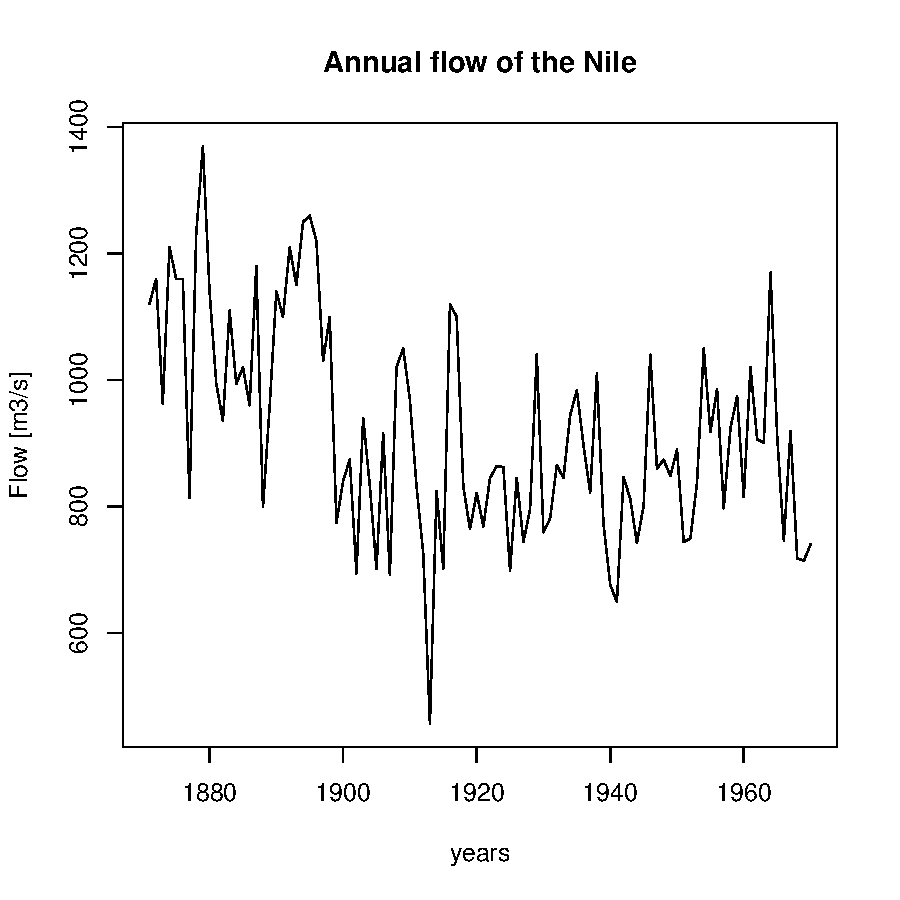
\includegraphics{alles-035}
\caption{Annual Flow of the Nile}
\end{figure}

\noindent Since there are annual observations, there is no indices of a cycle/ seasonality in the data. A non-seasonal time series consists of a trend and an irregular component. 
To estimate the trend component of a non-seasonal time series that can be described using an additive model, it is common to use a smoothing method, such as calculating the simple moving average of the time series.

\noindent The SMA() function in the “TTR” R package can be used to smooth time series data using a simple moving average. 
\begin{figure}
\centering
\begin{Schunk}
\begin{Sinput}
> library(TTR)
> plot(SMA(Nile,n=20))
> 
\end{Sinput}
\end{Schunk}
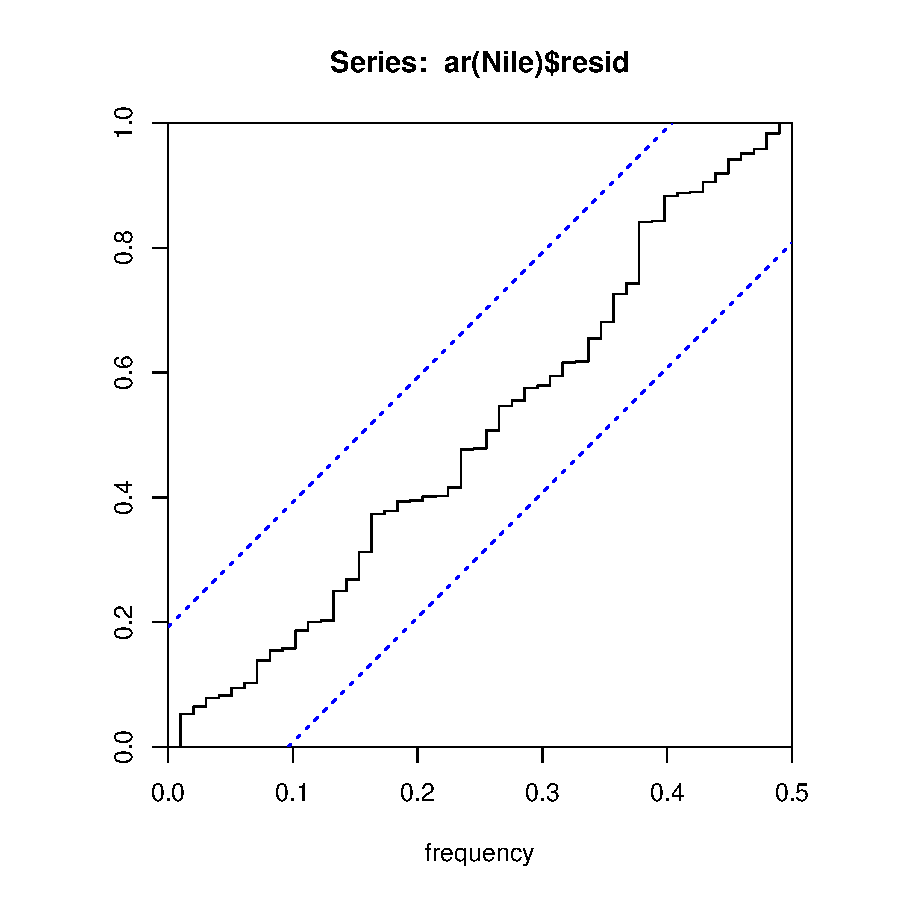
\includegraphics{alles-036}
\caption{Trend of the Annual Flow of the Nile}
\end{figure}

\noindent We can see that there was a negative trend until 1920 and that it becomes positiv since then. However it is difficult to make a clear statement of the trends, since there are high fluctuations in the data.\\


\noindent Now we can procede plotting the correlograms:
\begin{figure}
\centering
\begin{Schunk}
\begin{Sinput}
> par(mfrow = c(1, 2))
> acf(Nile)
> pacf(Nile)
> par(mfrow = c(1, 1))
\end{Sinput}
\end{Schunk}
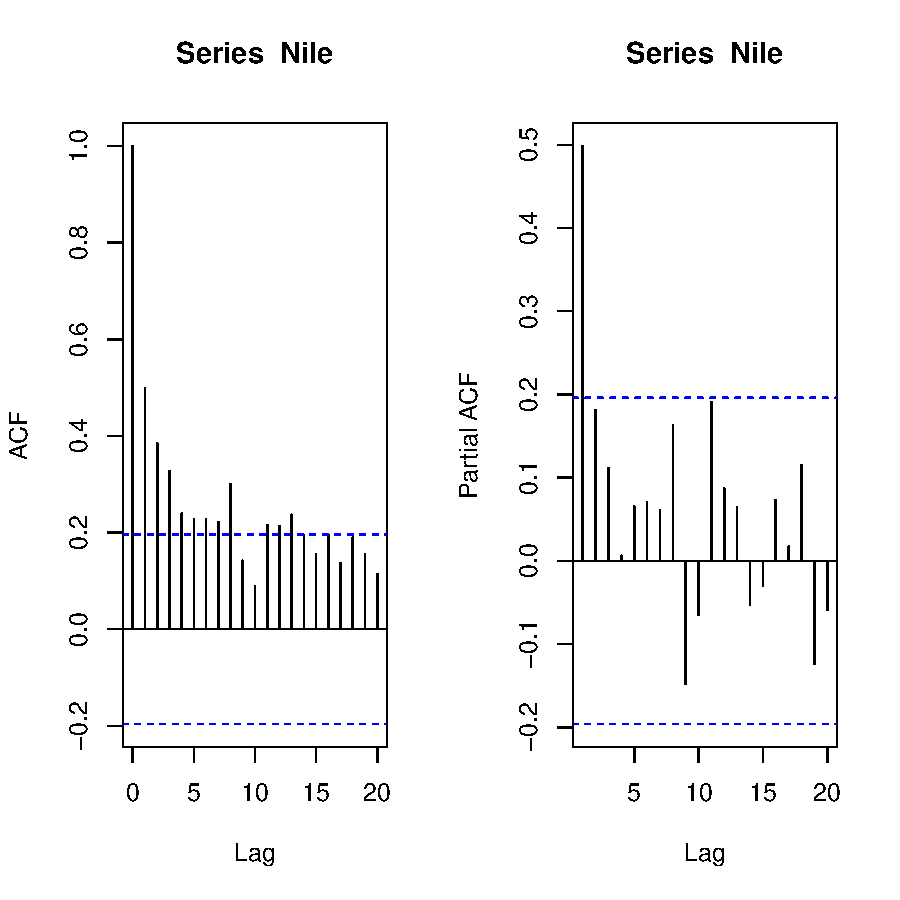
\includegraphics{alles-037}
\caption{Autocorrelations and Partial autocorrelations.}
\end{figure}

\noindent We find a significant autocorrelation at the first lags only, that means that the autocorrelation is not constanst over the time. 
At the Partial autocorrelation plot we do not observe a significant autocorrelation. 

\noindent We can first fit an autoregression model to the Nile Time Series:
\begin{figure}
\centering
\begin{Schunk}
\begin{Sinput}
> ar(Nile) # selects order 2
\end{Sinput}
\begin{Soutput}
Call:
ar(x = Nile)

Coefficients:
     1       2  
0.4081  0.1812  

Order selected 2  sigma^2 estimated as  21247
\end{Soutput}
\begin{Sinput}
> cpgram(ar(Nile)$resid)
> arima(Nile, c(2, 0, 0))
\end{Sinput}
\begin{Soutput}
Series: Nile 
ARIMA(2,0,0) with non-zero mean 

Coefficients:
         ar1     ar2  intercept
      0.4096  0.1987   919.8397
s.e.  0.0974  0.0990    35.6410

sigma^2 estimated as 20291:  log likelihood=-637.98
AIC=1283.96   AICc=1284.38   BIC=1294.38
\end{Soutput}
\begin{Sinput}
> 
\end{Sinput}
\end{Schunk}
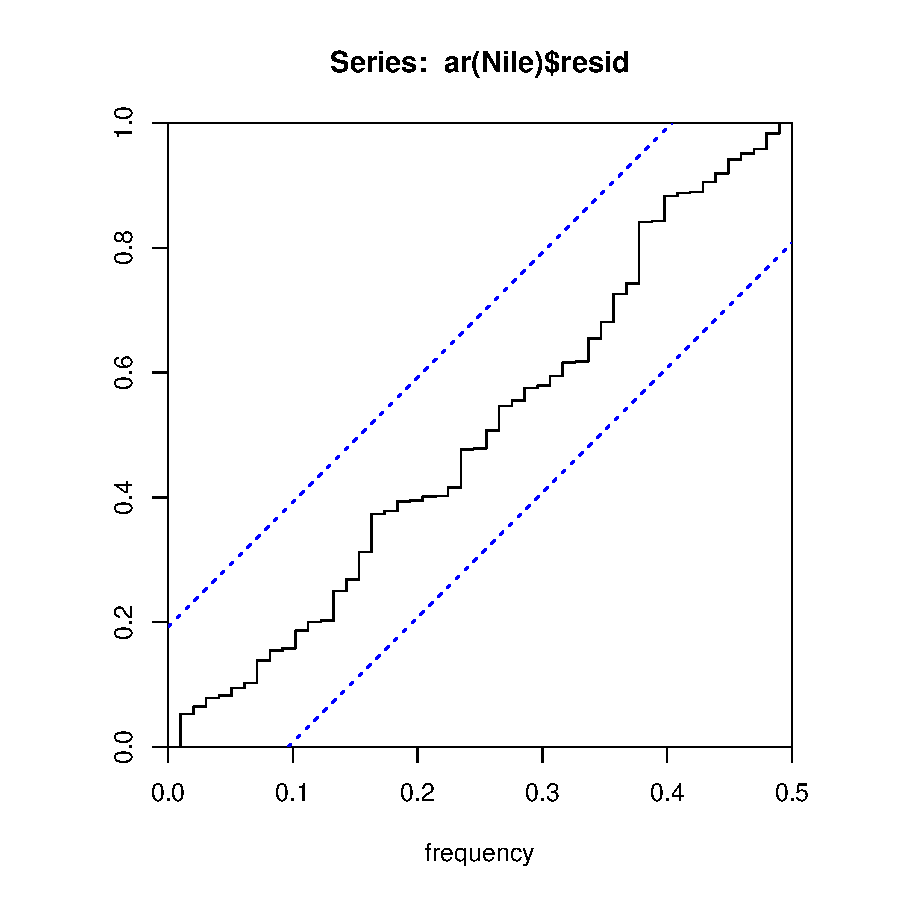
\includegraphics{alles-038}
\caption{Cumulative Peridiogram of the residuals}
\end{figure}

\noindent Fitting a autoregressive model, we can see that the residuals are well placed.

\subsubsection{Holt Winters exponential smoothing}

\begin{figure}
\centering
\begin{Schunk}
\begin{Sinput}
> library(forecast)
> hwn = HoltWinters(Nile,alpha = 0.2, beta = FALSE, gamma = FALSE)
> plot(hwn)
> 
\end{Sinput}
\end{Schunk}
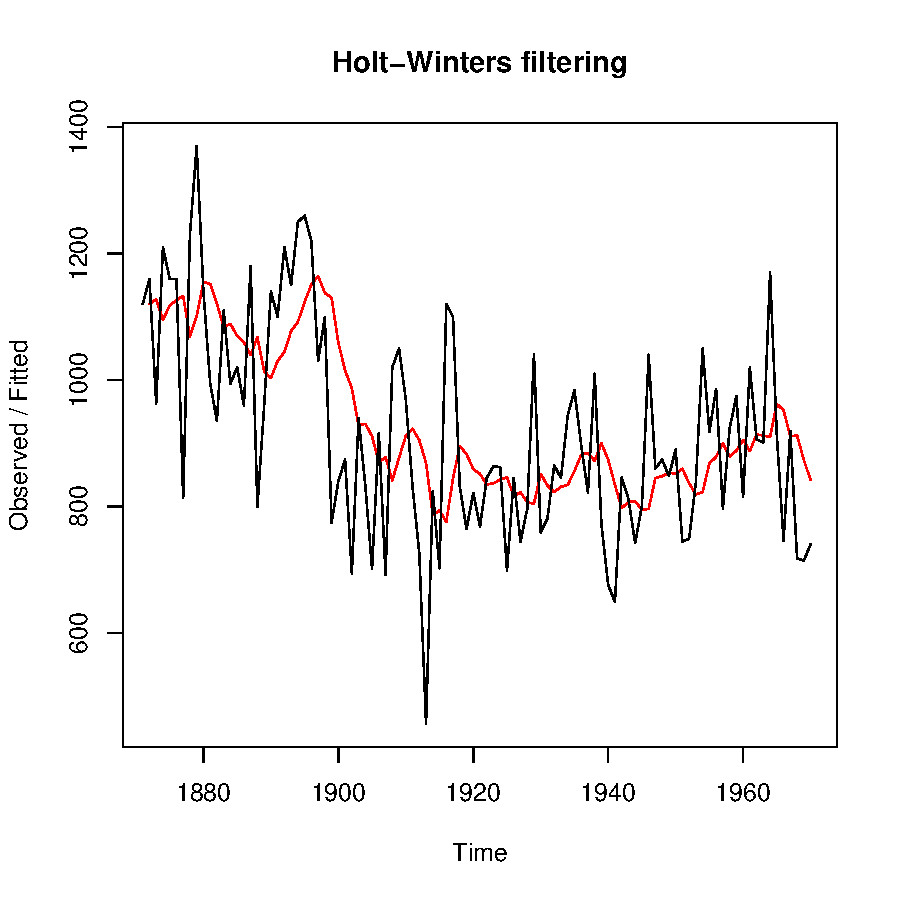
\includegraphics{alles-039}
\caption{Holt Winters}
\end{figure}

\begin{figure}
\centering
\begin{Schunk}
\begin{Sinput}
> forecast_nile = forecast.HoltWinters(hwn, h=10)
> plot.forecast(forecast_nile)
> 
\end{Sinput}
\end{Schunk}
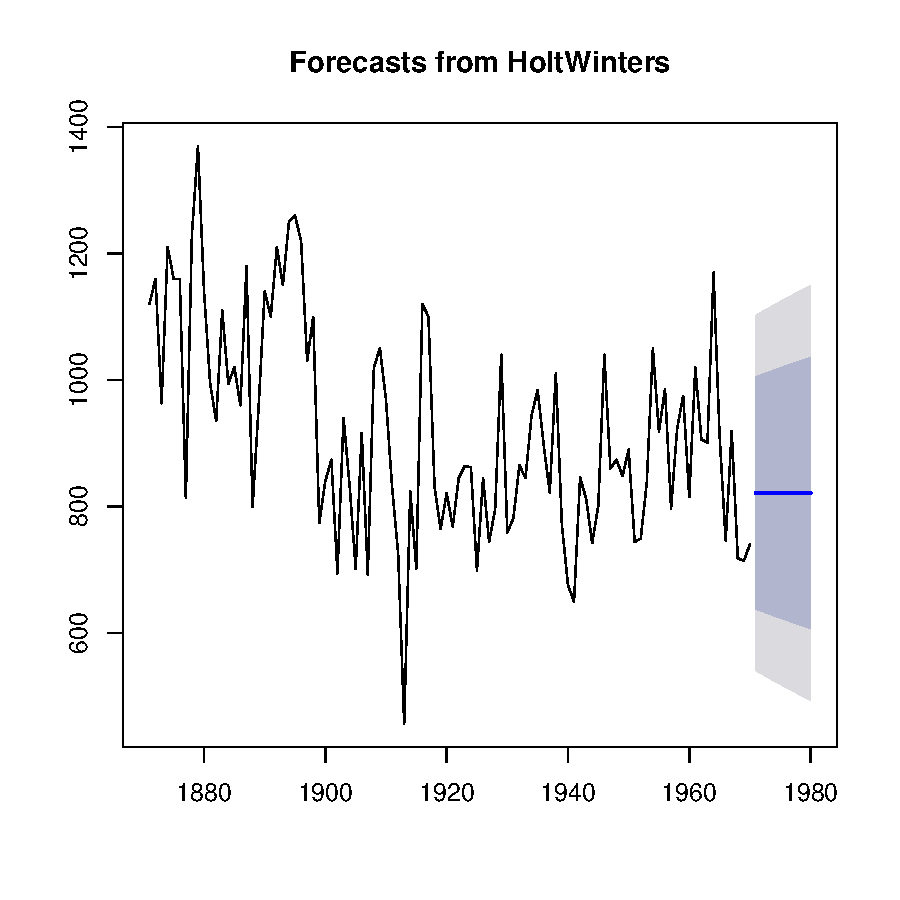
\includegraphics{alles-040}
\caption{Holt Winter Forecasting}
\end{figure}

\noindent The forecasts are shown as a blue line, with the 80% prediction intervals as an orange shaded area, and the 95% prediction intervals as a yellow shaded area.


\begin{Schunk}
\begin{Sinput}
> acf(forecast_nile$residuals, lag.max = 20)
> Box.test(forecast_nile$residuals, lag=20, type="Ljung-Box")
\end{Sinput}
\begin{Soutput}
	Box-Ljung test

data:  forecast_nile$residuals
X-squared = 15.8772, df = 20, p-value = 0.7242
\end{Soutput}
\begin{Sinput}
> 
\end{Sinput}
\end{Schunk}
\noindent At the Ljung-Box test the p-value is 0.85, indicating that there is little evidence of non-zero autocorrelations in the in-sample forecast errors at lags 1-20.

\noindent We should check that the forecast errors have constant variance over time, and are normally distributed with mean zero. We can do this by making a time plot of forecast errors, and a histogram of the distribution of forecast errors.



\begin{figure}
\centering
\begin{Schunk}
\begin{Sinput}
> par(mfrow=c(1,2))
> plot.ts(forecast_nile$residuals);abline(h=0)
> plotForecastErrors(forecast_nile$residuals)
\end{Sinput}
\end{Schunk}
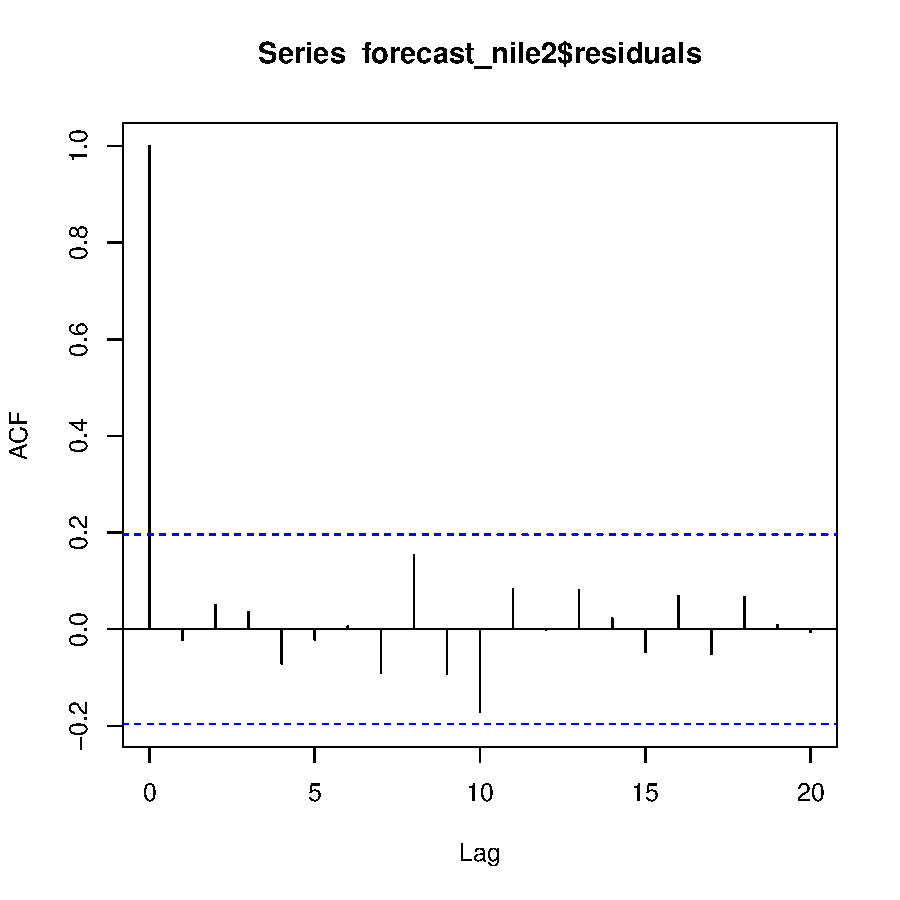
\includegraphics{alles-043}
\caption{Forecast Errors}
\end{figure}

\noindent The time plot of forecast errors shows that the forecast errors have roughly constant variance over time. The histogram of forecast errors show that it is plausible that the forecast errors are normally distributed with mean zero and constant variance.

\subsubsection{ARIMA}

\noindent While exponential smoothing methods do not make any assumptions about correlations between successive values of the time series, in some cases you can make a better predictive model by taking correlations in the data into account. Autoregressive Integrated Moving Average (ARIMA) models include an explicit statistical model for the irregular component of a time series, that allows for non-zero autocorrelations in the irregular component.
\begin{figure}
\centering
\begin{Schunk}
\begin{Sinput}
> nile_arima = auto.arima(Nile)
> forecast_nile2 = forecast.Arima(nile_arima, h=10)
> plot.forecast(forecast_nile2)
> 
\end{Sinput}
\end{Schunk}
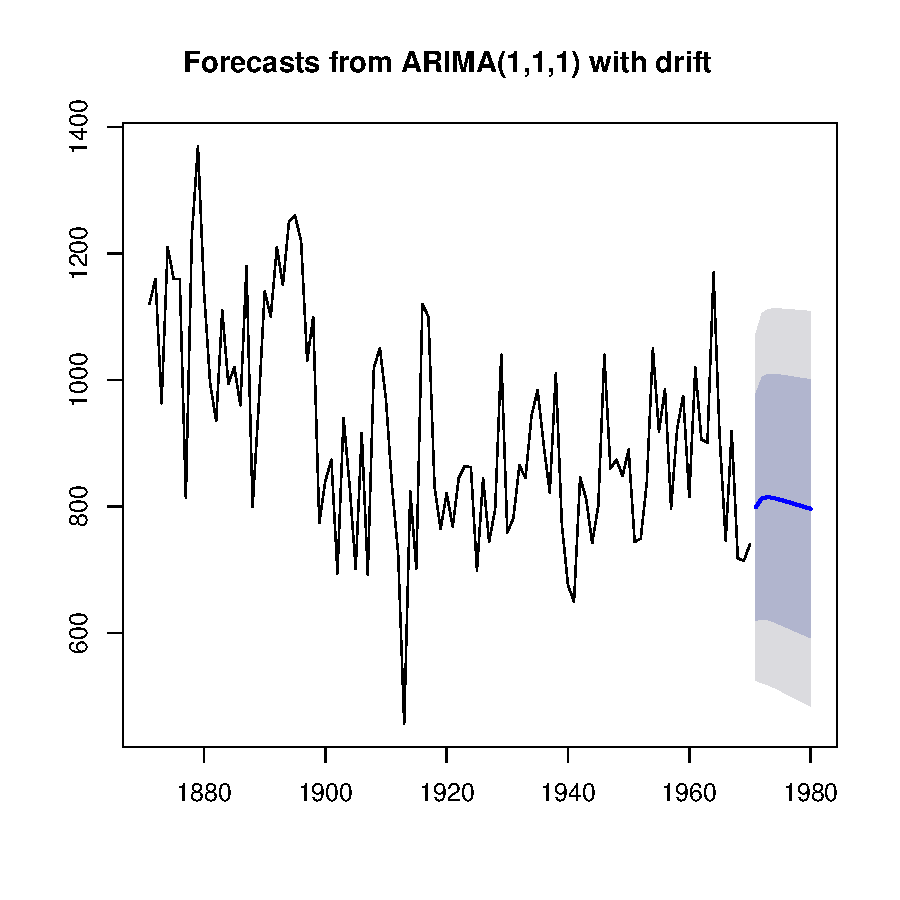
\includegraphics{alles-044}
\caption{Arima forecasting}
\end{figure}

Check for autocorrelations:
\begin{figure}
\centering
\begin{Schunk}
\begin{Sinput}
> acf(forecast_nile2$residuals, lag.max = 20)
> Box.test(forecast_nile2$residuals, lag=20, type="Ljung-Box")
\end{Sinput}
\begin{Soutput}
	Box-Ljung test

data:  forecast_nile2$residuals
X-squared = 12.1156, df = 20, p-value = 0.912
\end{Soutput}
\end{Schunk}
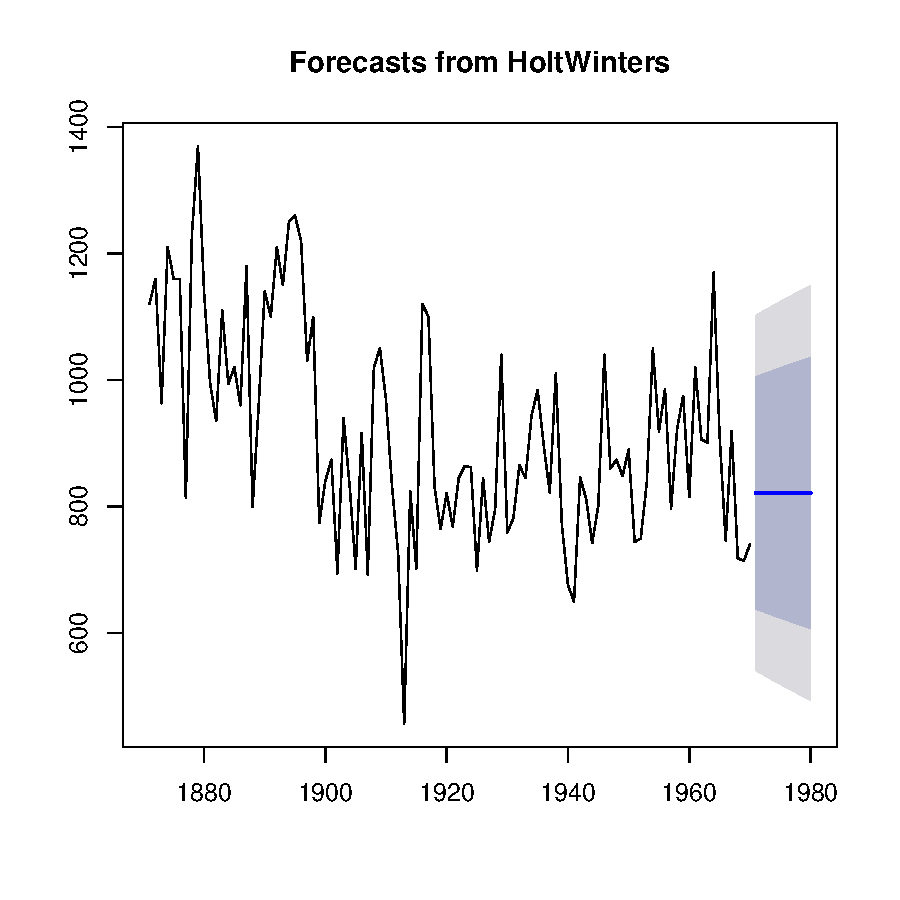
\includegraphics{alles-045}
\caption{acf of the residuals}
\end{figure}

\begin{figure}
\centering
\begin{Schunk}
\begin{Sinput}
> par(mfrow=c(1,2))
> plot.ts(forecast_nile2$residuals); abline(h=0)
> plotForecastErrors(forecast_nile2$residuals)
\end{Sinput}
\end{Schunk}
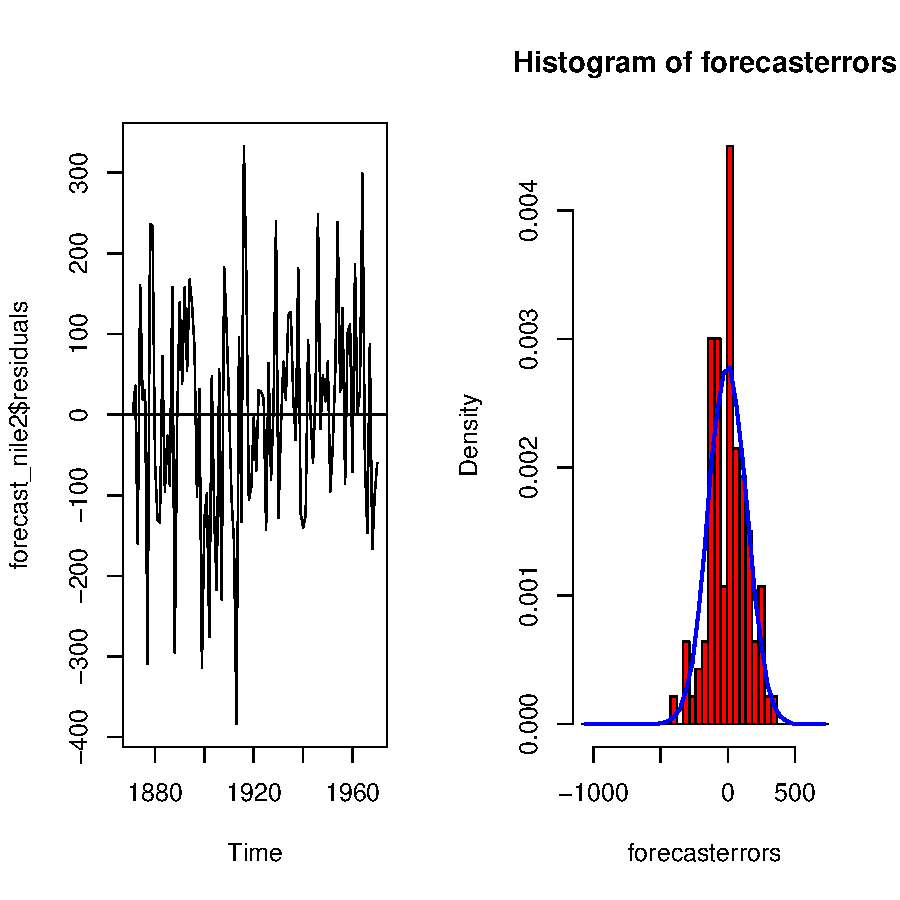
\includegraphics{alles-046}
\caption{Residuals and Errors}
\end{figure}

\begin{Schunk}
\begin{Sinput}
> nilelm = lm(Nile~time(Nile))
> summary(nilelm)
\end{Sinput}
\begin{Soutput}
Call:
lm(formula = Nile ~ time(Nile))

Residuals:
    Min      1Q  Median      3Q     Max 
-483.71  -98.17  -23.21  111.40  368.72 

Coefficients:
             Estimate Std. Error t value Pr(>|t|)    
(Intercept) 6132.1736  1001.7578   6.121 1.92e-08 ***
time(Nile)    -2.7143     0.5216  -5.204 1.07e-06 ***
---
Signif. codes:  0 '***' 0.001 '**' 0.01 '*' 0.05 '.' 0.1 ' ' 1

Residual standard error: 150.6 on 98 degrees of freedom
Multiple R-squared:  0.2165,	Adjusted R-squared:  0.2085 
F-statistic: 27.08 on 1 and 98 DF,  p-value: 1.072e-06
\end{Soutput}
\begin{Sinput}
> acf(resid(nilelm))
> pacf(resid(nilelm))
\end{Sinput}
\end{Schunk}


\begin{Schunk}
\begin{Sinput}
> library(nlme)
> nilegls = gls(Nile ~ time(Nile),cor= corAR1(acf(resid(nilelm))$acf[2]))
> save(nilegls, file="nilegls.RData")
> 
> 
\end{Sinput}
\end{Schunk}


\begin{Schunk}
\begin{Sinput}
> load("nilegls.RData")
\end{Sinput}
\end{Schunk}


\begin{Schunk}
\begin{Sinput}
> acf(nilegls$residuals, plot = F)
> summary(nilegls)
\end{Sinput}
\begin{Soutput}
Generalized least squares fit by REML
  Model: Nile ~ time(Nile) 
  Data: NULL 
       AIC      BIC    logLik
  1268.205 1278.545 -630.1026

Correlation Structure: AR(1)
 Formula: ~1 
 Parameter estimate(s):
      Phi 
0.4002726 

Coefficients:
               Value Std.Error   t-value p-value
(Intercept) 6216.491 1518.1486  4.094784   1e-04
time(Nile)    -2.758    0.7904 -3.489523   7e-04

 Correlation: 
           (Intr)
time(Nile) -1    

Standardized residuals:
       Min         Q1        Med         Q3        Max 
-3.1787691 -0.6428562 -0.1463738  0.7245317  2.4323739 

Residual standard error: 152.3157 
Degrees of freedom: 100 total; 98 residual
\end{Soutput}
\begin{Sinput}
> confint(nilegls)
\end{Sinput}
\begin{Soutput}
                  2.5 %      97.5 %
(Intercept) 3240.974234 9192.007340
time(Nile)    -4.307301   -1.208971
\end{Soutput}
\begin{Sinput}
> plot(nilegls)
> plot(nilelm)
\end{Sinput}
\end{Schunk}



\begin{Schunk}
\begin{Sinput}
> Box.test(nilegls$residuals, type="Ljung-Box")
\end{Sinput}
\begin{Soutput}
	Box-Ljung test

data:  nilegls$residuals
X-squared = 14.496, df = 1, p-value = 0.0001405
\end{Soutput}
\end{Schunk}
\noindent The NULL-Hypothesis can be rejected, the residuals are not independent. 

\noindent We can check which model has the best AIC:
\begin{Schunk}
\begin{Sinput}
> AIC(nilelm)
\end{Sinput}
\begin{Soutput}
[1] 1290.629
\end{Soutput}
\begin{Sinput}
> AIC(nilegls)
\end{Sinput}
\begin{Soutput}
[1] 1268.205
\end{Soutput}
\end{Schunk}
\noindent The nilegls Model seems to be better.

\noindent And we perform the Durbin Watson Test to check for autocorrelations.
\begin{Schunk}
\begin{Sinput}
> library(car)
> dwt(as.vector(nilegls$residuals)) 
\end{Sinput}
\begin{Soutput}
[1] 1.247133
\end{Soutput}
\end{Schunk}
\noindent The Durbin Watson Test of the residuals shows that there is no autocorrelation.


\subsubsection{Structural time series models}

\noindent The function StructTS fits a model by maximum likelihood.
\begin{Schunk}
\begin{Sinput}
> fit <- StructTS(Nile, type = "level")
> fit
\end{Sinput}
\begin{Soutput}
Call:
StructTS(x = Nile, type = "level")

Variances:
  level  epsilon  
   1469    15099  
\end{Soutput}
\end{Schunk}
\noindent The maximum likelihood estimates (MLEs) of the level and observation error variances, 1469 and 15099, respectively, are included in the output as the coefficients of fit. 

\begin{figure}
\centering
\begin{Schunk}
\begin{Sinput}
> par(mfrow = c(3, 1))
> plot(Nile)
> ## local level model
> lines(fitted(fit), lty = "dashed", col=4)       # contemporaneous smoothing
> lines(tsSmooth(fit), lty = "dotted", col = 6)   # fixed-interval smoothing
> legend("bottomright" ,col = c(4,6),c("filtered","smoothed"), lty=c("dashed", "dotted"), bty="n", cex=0.8)
> plot(residuals(fit)); abline(h = 0, lty = 3)
> ## local trend model
> (fit2 <- StructTS(Nile, type = "trend")) ## constant trend fitted
\end{Sinput}
\begin{Soutput}
Call:
StructTS(x = Nile, type = "trend")

Variances:
  level    slope  epsilon  
   1427        0    15047  
\end{Soutput}
\begin{Sinput}
> pred <- predict(fit, n.ahead = 30)
> ## with 95% confidence interval
> ts.plot(Nile, pred$pred,
+         pred$pred + 1.96*pred$se, pred$pred -1.96*pred$se, col=c(1,2,1))
> par(mfrow=c(1,1))
> 
\end{Sinput}
\end{Schunk}
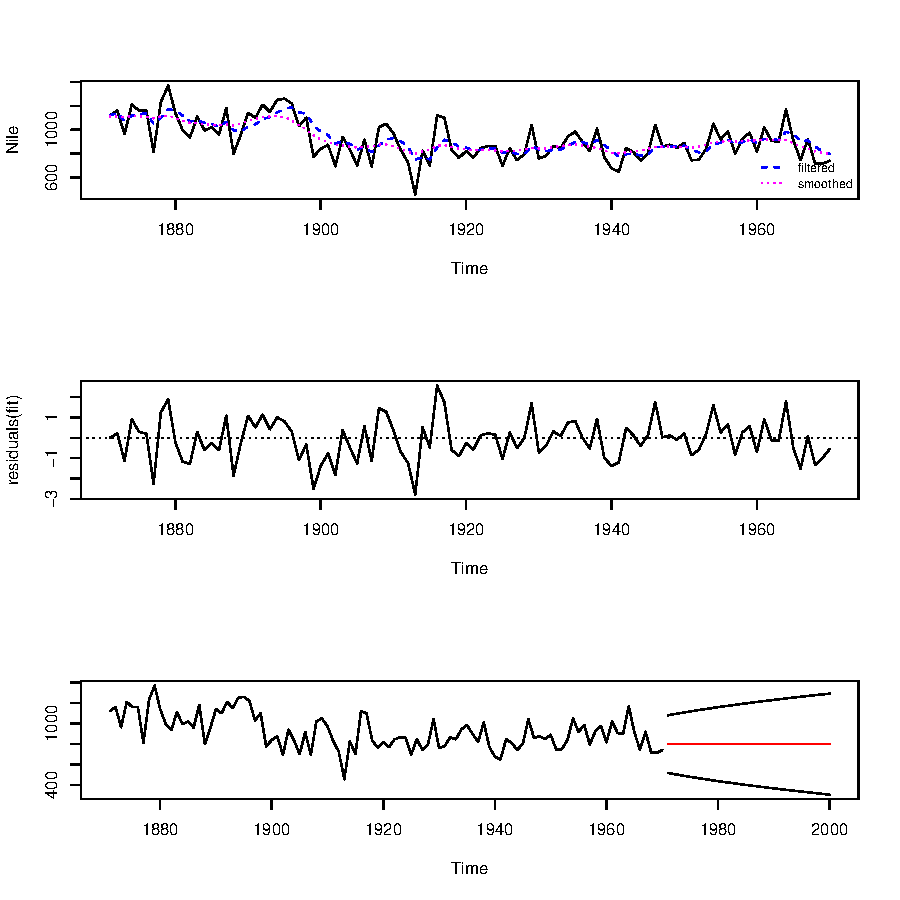
\includegraphics{alles-055}
\caption{Fitting a Structural Model}
\end{figure}

\noindent The function tsdiag can be called on an object of class StructTS to obtain diagnostic plots based on the standardized one-step-ahead forecast errors.
\begin{figure}
\centering
\begin{Schunk}
\begin{Sinput}
> tsdiag(fit)
> tsdiag(fit2)
> 
\end{Sinput}
\end{Schunk}
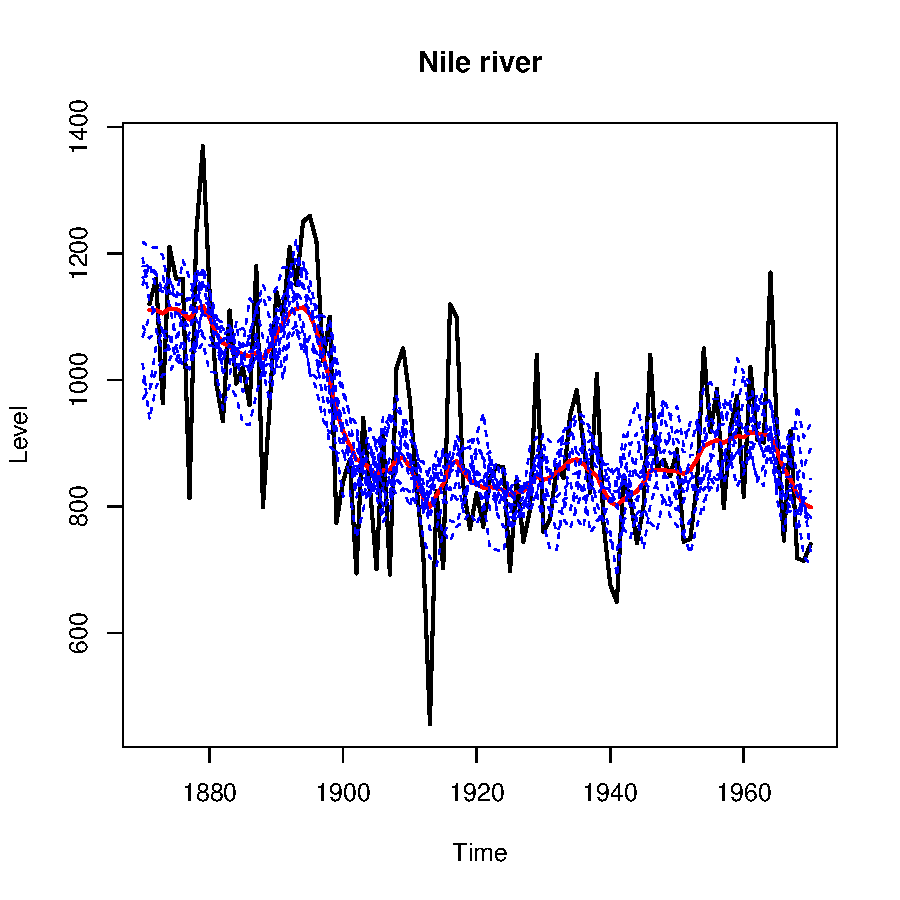
\includegraphics{alles-056}
\caption{Models diagnostics}
\end{figure}

\noindent Forecasts for structural time series, as objects of class StructTS, can be obtained by either the method function predict or forecast in package forecast (Hyndman 2011; Hyndman and Khandakar 2008). This package provides also a convenient plot method function for the resulting object of class forecast. Figure \ref{Forecasted values}, obtained with the code below, shows the forecasted Nile river data until 1980, togeher with 50% and 90% probability intervals.

\begin{figure}
\centering
\begin{Schunk}
\begin{Sinput}
> library(forecast)
> plot(forecast(fit2, level = c(50,90), h = 10), xlim = c(1950, 1980), shadecols = "oldstyle")
\end{Sinput}
\end{Schunk}
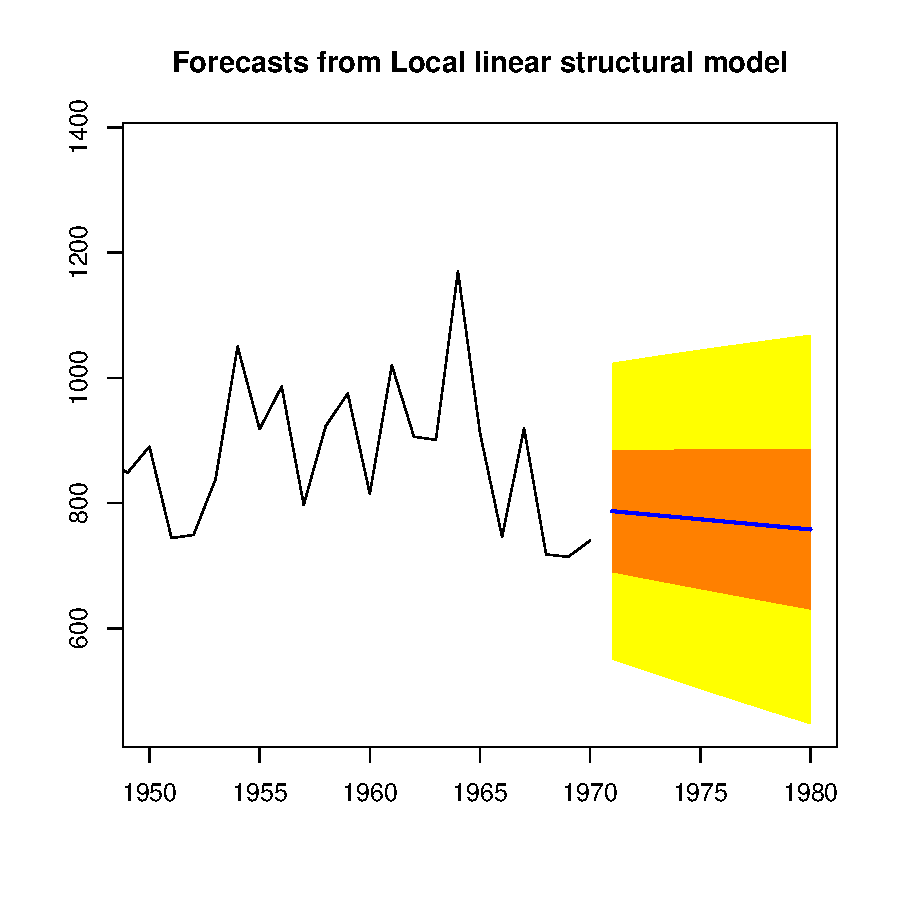
\includegraphics{alles-Forecasted values}
\caption{Forecasted values}
\end{figure}

\subsubsection{The local level model with package dlm }
\noindent A polynomial DLM (a local level model is a polynomial DLM of order 1, a local linear trend is a polynomial DLM of order 2), is easily defined in dlm through the function dlmModPoly.The function simulates one draw from the posterior distribution of the state vectors.

\begin{figure}
\centering
\begin{Schunk}
\begin{Sinput}
> library(dlm)
> nile_mod <- dlmModPoly(1, dV = 15099.8, dW = 1468.4) #values taken from the coefficients of fit
> nile_filt <- dlmFilter(Nile, nile_mod)
> nile_smooth <- dlmSmooth(nile_filt) # estimated "true" level
> plot(cbind(Nile, nile_smooth$s[-1]), plot.type = "s",
+      col = c("black", "red"), ylab = "Level",
+      main = "Nile river", lwd = c(2, 2)) 
> for (i in 1:10) # 10 simulated "true" levels 
+     lines(dlmBSample(nile_filt[-1]), lty=2, col="blue")
\end{Sinput}
\end{Schunk}
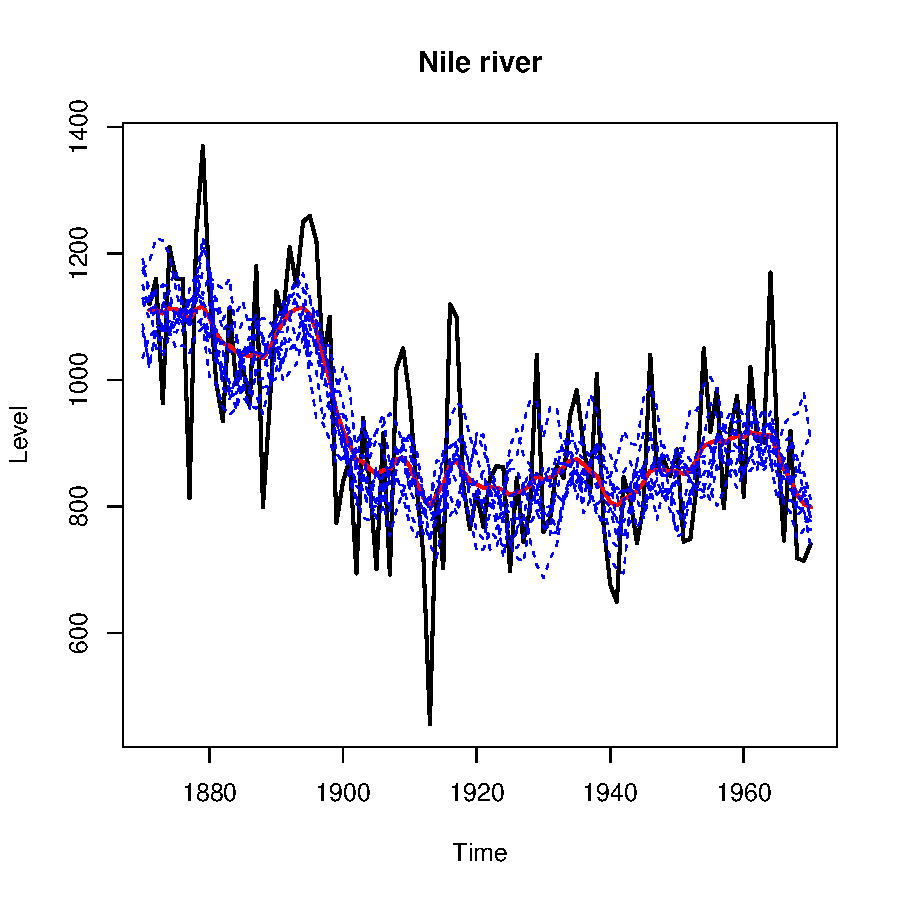
\includegraphics{alles-058}
\caption{dlm Model}
\end{figure}

\subsection

library(mgcv)
niletime = time(Nile)
gamnile = gam(as.numeric(Nile) ~ s(niletime),cor=corARMA(p=2, q=0)) 
plot.gam(gamnile,residuals = T, se=T, main="GAM-Model")





\section{compabitily with linux and other computers}


\section{Links and Further Reading}%-----------------------------------------------------------------------------------------------
and in:\\
http://cran.r-project.org/web/views/TimeSeries.html\\
Another Exemple Datasets are avaliable at:\\
http://www.comp-engine.org/timeseries/browse-data-by-category\\
https://datamarket.com/data/list/?q=provider:tsdl\\
\section{Acknowledgements}%------------------------------------------------------------------------------------------------------
Don't forget to thank TeX and R and other opensource communities if you use their products! The correct way to cite R is shown when typing ``\texttt{citation()}'', and ``\texttt{citation("mgcv")}'' for packages.
\clearpage
\end{document}
